% Provenance (never printed): old premiere S / seconde material on minerals and
% rocks (identifying minerals in hand specimen, the silicates, the minerals of
% granite, basalt and peridotite, thin sections in polarised light).
% Element fractions and rock densities from figdata/grade-11/mineral_density.py
% (Rudnick and Gao 2014 bulk crust; webmineral mean densities). Mineral, crystal,
% rock families and the Mohs scale are Book 1's (grade 6): recalled, not defined.
% Felsic and mafic belong to g11.08: not used here.
\chapter{खनिज}\label{ch:g11:minerals}

ग्रेनाइट का एक कंकड़ उठाइए और उसे हाथ-लेंस से देखिए। वह एक पदार्थ नहीं,
बल्कि आपस में जकड़े कणों की पच्चीकारी है: धूसर कण, काँच जैसे और
लगभग पारदर्शी; गुलाबी कण, खंड जैसे, जिनके टूटे फलक कंकड़ घुमाने पर
रोशनी में चमक उठते हैं; छोटी काली पपड़ियाँ जिन्हें चाकू की नोक पतली
परतों में उठा देती है। हर प्रकार का कण एक खनिज है। यह अध्याय दिखाता है कि
भूवैज्ञानिक उन्हें कैसे अलग पहचानता है, लगभग सभी सिलिकन
और ऑक्सीजन से क्यों बने हैं, वे अब तक मिली चट्टानें --- ग्रेनाइट, बेसाल्ट,
\omterm{def:g11:ocean-ridges:peridotite}{पेरिडोटाइट} --- कैसे बनाते हैं, और बाल से भी पतली चट्टान की एक फाँक, ध्रुवित
प्रकाश में देखने पर, उन सबको एक साथ कैसे दिखाती है।

\begin{omfigure}
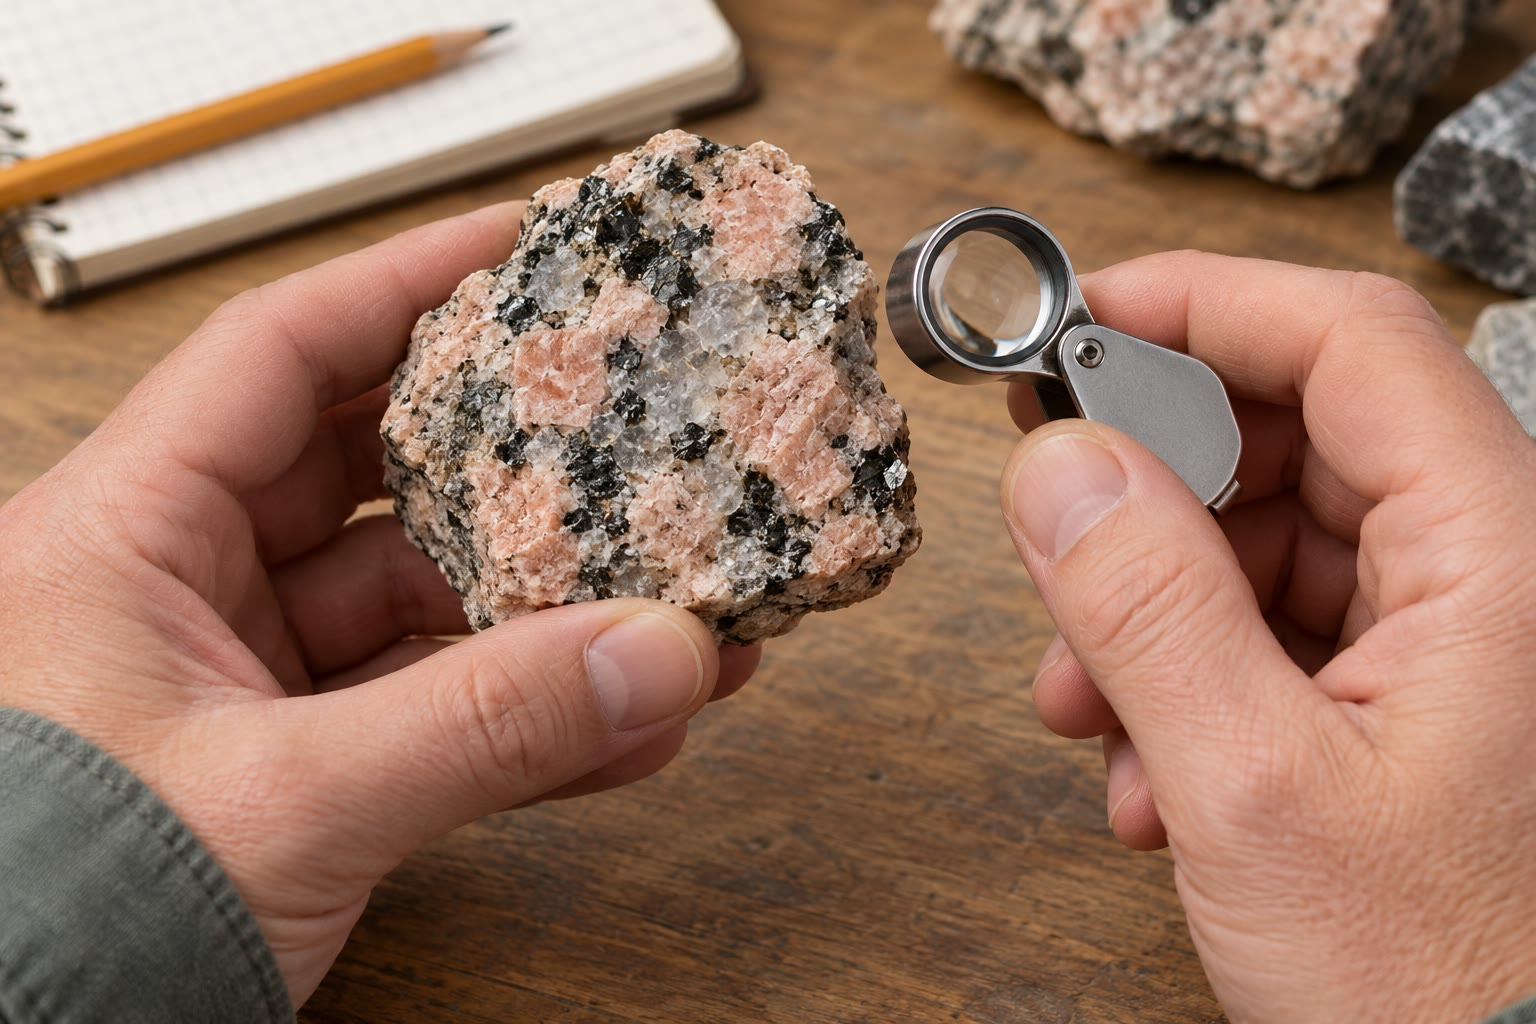
\includegraphics[width=0.62\linewidth]{images/book2/ai/g11-geologist-hand-lens.jpg}

{\small हाथ-लेंस से जाँचा जाता एक ग्रेनाइट: खनिजों को अलग पहचानने का
पहला औज़ार। (AI द्वारा बनाया गया चित्र।)}
\end{omfigure}

\begin{recall}
खनिज एक प्राकृतिक ठोस पदार्थ है, जिसे जीवों ने नहीं बनाया, जिसकी
बनावट निश्चित है और जिसके परमाणु एक नियमित ढंग से व्यवस्थित हैं; चट्टान एक
या कई खनिजों से बनी होती है। ग्रेनाइट ज़्यादातर फ़ेल्डस्पार, क्वार्ट्ज़ और अभ्रक से बना है।
चट्टानें तीन परिवारों में बँटती हैं: आग्नेय, अवसादी और कायांतरित। किसी
खनिज की कठोरता यह है कि वह खरोंचे जाने का कितना अच्छा विरोध करता है, जिसे मोह्स पैमाने पर 1
(टैल्क) से 10 (हीरा) तक क्रम दिया जाता है; ऑर्थोक्लेज़ फ़ेल्डस्पार 6 है और क्वार्ट्ज़
7, जबकि काँच की प्लेट लगभग 5.5 है और स्टील की कील लगभग 6.5 (पुस्तक 1,
कक्षा 6)। किसी पिंड का घनत्व उसका द्रव्यमान बटा उसका आयतन है
(भौतिकी)। किसी यौगिक का वर्णन एक सूत्र से होता है जो उसके परमाणु गिनता है; आयनों से बने
ठोस में धनात्मक और ऋणात्मक आवेश संतुलित होते हैं (रसायन)।
\omterm{def:g11:ocean-ridges:peridotite}{पेरिडोटाइट} प्रावार बनाता है; \omterm{def:g11:ocean-ridges:gabbro}{गैब्रो} और बेसाल्ट \omterm{def:g11:ocean-ridges:oceanic-lithosphere}{महासागरीय भूपर्पटी} बनाते हैं
(\cref{ch:g11:ocean-ridges})।
\end{recall}
% ledger: usgs:mineral-rock, nps:granite-minerals, nps:mohs-ladder, nps:mohs-testers

\section{खनिजों को अलग पहचानना}

खनिज की बनावट निश्चित होती है और उसके परमाणुओं की व्यवस्था नियमित। दोनों
बाहर से दिखती हैं: उसके क्रिस्टलों की आकृति में, उसके टूटने के ढंग में, उसके
प्रकाश परावर्तित करने के ढंग में, उसकी कठोरता और उसके घनत्व में। इनमें से कोई भी गुण
अकेला पर्याप्त नहीं; मिलकर वे हस्त-नमूने में सामान्य खनिजों को पहचान लेते हैं,
बिना किसी उपकरण के, केवल एक लेंस, स्टील की एक कील और काँच की एक प्लेट से।

\paragraph{आकृति।} जो क्रिस्टल किसी खोखले में या किसी द्रव में खुलकर बढ़ा,
वह ऐसी आकृति लेता है जो उसके परमाणुओं की व्यवस्था को दर्शाती है।

\begin{definition}[स्वभाव]\label{def:g11:minerals:habit}
किसी खनिज का \emph{स्वभाव}\index{स्वभाव (क्रिस्टल का)} वह सामान्य आकृति है
जो उसके क्रिस्टल लेते हैं: घनाकार, पट्टिकाकार (पट्टी की तरह चपटा), प्रिज़्माकार
(प्रिज़्म की तरह लंबा), फलकाकार, सूच्याकार (सुई जैसा), इत्यादि।
\end{definition}
% ledger: tulane:physprop

क्वार्ट्ज़ नुकीले सिरों वाले षट्भुजीय प्रिज़्मों के रूप में बढ़ता है; बायोटाइट, चपटी
षट्भुजीय प्लेटों के रूप में (नीचे की फ़ोटो)। फिर भी अधिकांश चट्टानों में कण
एक-दूसरे से सटकर बढ़े हैं और उनके अपने कोई फलक नहीं हैं: तब \omterm{def:g11:minerals:habit}{स्वभाव} कम बताता है,
और दूसरे गुण काम सँभालते हैं।
% ledger: photo:g11-quartz, photo:g11-biotite

\paragraph{रंग और द्युति।} रंग वह पहली चीज़ है जो दिखती है, और सबसे
कम भरोसेमंद। किसी दूसरे तत्त्व का अंश मात्र उसे बदलने के लिए काफ़ी है: क्वार्ट्ज़
पारदर्शी, सफ़ेद, काला, गुलाबी, नीला या बैंगनी हो सकता है। दूसरी ओर, कुछ खनिज
मुश्किल से बदलते हैं: ओलिवीन लगभग हमेशा हरा होता है। खनिज प्रकाश को
कैसे परावर्तित करता है, यह बेहतर मार्गदर्शक है।
% ledger: tulane:physprop

\begin{definition}[द्युति]\label{def:g11:minerals:lustre}
किसी खनिज की \emph{द्युति}\index{द्युति} परावर्तित प्रकाश में उसका रूप है।
जब खनिज धातु की तरह चमकता है तो वह \emph{धात्विक} होती है, और
अन्यथा अधात्विक: \emph{काचाभ} (क्वार्ट्ज़ की तरह काँच जैसी), मुक्ताभ,
रालाभ, इत्यादि।
\end{definition}
% ledger: tulane:physprop

\paragraph{टूटने का ढंग।} क्रिस्टल पर चोट कीजिए और वह टूट जाता है। जहाँ
उसके परमाणुओं के बीच के बंध कुछ तलों के अनुदिश कमज़ोर होते हैं, वह उनके अनुदिश,
बार-बार, समतल चमकीली सतहों में फटता है; जहाँ कोई तल दूसरे से
कमज़ोर नहीं होता, वह किसी भी सतह के अनुदिश टूटता है।

\begin{definition}[विदलन; विभंग]\label{def:g11:minerals:cleavage}
\emph{विदलन}\index{विदलन (खनिज का)} किसी खनिज की समतल तलों के अनुदिश टूटने की
प्रवृत्ति है, जो उन दिशाओं के समांतर होते हैं जिनमें उसके परमाणुओं के बीच के बंध
कमज़ोर हैं। \emph{विभंग}\index{विभंग (खनिज का)}
अनियमित सतहों के अनुदिश टूटना है, ऐसे खनिज में जिसमें कोई कमज़ोर तल
नहीं; टूटे काँच जैसी चिकनी वक्र सतहों वाला विभंग
\emph{शंखाभ} कहलाता है।
\end{definition}
% ledger: tulane:physprop

किसी खनिज का एक \omterm{def:g11:minerals:cleavage}{विदलन} हो सकता है, दो, तीन या कोई नहीं। अभ्रकों का एक होता है, पूर्ण:
वे परतों में उतरते हैं। फ़ेल्डस्पारों के दो होते हैं। क्वार्ट्ज़ का कोई नहीं: वह
शंखाभ \omterm{def:g11:minerals:cleavage}{विभंग} के साथ टूटता है, जिससे वह उसी धूसर या सफ़ेद रंग के फ़ेल्डस्पार से
तुरंत अलग पहचाना जाता है। दो \omterm{def:g11:minerals:cleavage}{विदलनों} के बीच का कोण परमाणुओं की व्यवस्था से
तय होता है, और उसे किसी टूटे कण या किसी काट पर मापा जा सकता है: पाइरॉक्सीन के दो
\omterm{def:g11:minerals:cleavage}{विदलन} लगभग \ang{87} और \ang{93} पर मिलते हैं, लगभग समकोण;
ऐम्फ़िबोल के लगभग \ang{56} और \ang{124} पर। पाइरॉक्सीन और
ऐम्फ़िबोल अक्सर गहरे रंग के और एक जैसे होते हैं; उनके विदलन-कोण उन्हें अलग करते हैं।
% ledger: wm:densities (quartz conchoidal; orthoclase two cleavages; biotite one), tulane:cleavage-angles

\begin{omfigure}
\begin{tikzpicture}[font=\footnotesize]
  % pyroxene: octagonal cross-section, cleavage traces at 46.5 and 133.5 degrees (87/93)
  \begin{scope}
    \coordinate (p1) at (1,0.4); \coordinate (p2) at (0.431,1); \coordinate (p3) at (-0.431,1);
    \coordinate (p4) at (-1,0.4); \coordinate (p5) at (-1,-0.4); \coordinate (p6) at (-0.431,-1);
    \coordinate (p7) at (0.431,-1); \coordinate (p8) at (1,-0.4);
    \begin{scope}[scale=1.5]
      \fill[black!72!green!40] (1,0.4) -- (0.431,1) -- (-0.431,1) -- (-1,0.4) -- (-1,-0.4) -- (-0.431,-1) -- (0.431,-1) -- (1,-0.4) -- cycle;
      \clip (1,0.4) -- (0.431,1) -- (-0.431,1) -- (-1,0.4) -- (-1,-0.4) -- (-0.431,-1) -- (0.431,-1) -- (1,-0.4) -- cycle;
      \foreach \s in {-5,...,5} {
        \draw[white!85!black, line width=0.5pt] ($(136.5:\s*0.24)+(46.5:-3)$) -- ($(136.5:\s*0.24)+(46.5:3)$);
        \draw[white!85!black, line width=0.5pt] ($(223.5:\s*0.24)+(133.5:-3)$) -- ($(223.5:\s*0.24)+(133.5:3)$);}
      \draw[black!80, line width=0.9pt] (46.5:-3) -- (46.5:3); \draw[black!80, line width=0.9pt] (133.5:-3) -- (133.5:3);
    \end{scope}
    \draw[black!70, line width=0.7pt, scale=1.5] (1,0.4) -- (0.431,1) -- (-0.431,1) -- (-1,0.4) -- (-1,-0.4) -- (-0.431,-1) -- (0.431,-1) -- (1,-0.4) -- cycle;
    \draw[omProp, line width=1pt] (46.5:0.75) arc[start angle=46.5, end angle=133.5, radius=0.75];
    \draw[omDef, line width=1pt] (133.5:0.5) arc[start angle=133.5, end angle=226.5, radius=0.5];
    \node[fill=white, inner sep=1pt, text=omProp!80!black] at (90:0.98) {\ang{87}};
    \node[fill=white, inner sep=1pt, text=omDef] at (180:0.82) {\ang{93}};
    \node[anchor=north, align=center] at (0,-1.7) {\strut\textbf{पाइरॉक्सीन}\\विदलन लगभग \ang{87} और \ang{93} पर};
  \end{scope}
  % amphibole: elongated hexagon, cleavage traces at 28 and 152 degrees (56/124 opening sideways)
  \begin{scope}[xshift=6.2cm]
    \begin{scope}[scale=1.5]
      \fill[black!72!green!40] (1.6,0) -- (0.62,0.52) -- (-0.62,0.52) -- (-1.6,0) -- (-0.62,-0.52) -- (0.62,-0.52) -- cycle;
      \clip (1.6,0) -- (0.62,0.52) -- (-0.62,0.52) -- (-1.6,0) -- (-0.62,-0.52) -- (0.62,-0.52) -- cycle;
      \foreach \s in {-6,...,6} {
        \draw[white!85!black, line width=0.5pt] ($(118:\s*0.2)+(28:-4)$) -- ($(118:\s*0.2)+(28:4)$);
        \draw[white!85!black, line width=0.5pt] ($(242:\s*0.2)+(152:-4)$) -- ($(242:\s*0.2)+(152:4)$);}
      \draw[black!80, line width=0.9pt] (28:-4) -- (28:4); \draw[black!80, line width=0.9pt] (152:-4) -- (152:4);
    \end{scope}
    \draw[black!70, line width=0.7pt, scale=1.5] (1.6,0) -- (0.62,0.52) -- (-0.62,0.52) -- (-1.6,0) -- (-0.62,-0.52) -- (0.62,-0.52) -- cycle;
    \draw[omProp, line width=1pt] (-28:0.75) arc[start angle=-28, end angle=28, radius=0.75];
    \draw[omDef, line width=1pt] (28:0.42) arc[start angle=28, end angle=152, radius=0.42];
    \node[fill=white, inner sep=1pt, text=omProp!80!black] at (0:1.02) {\ang{56}};
    \node[fill=white, inner sep=1pt, text=omDef] at (90:0.6) {\ang{124}};
    \node[anchor=north, align=center] at (0,-1.7) {\strut\textbf{ऐम्फ़िबोल}\\विदलन लगभग \ang{56} और \ang{124} पर};
  \end{scope}
\end{tikzpicture}

{\small पाइरॉक्सीन के एक क्रिस्टल (बाएँ) और ऐम्फ़िबोल के एक क्रिस्टल
(दाएँ) की अनुप्रस्थ काटें, उनकी लंबाई के आर-पार काटी गईं (चित्र)। पतली रेखाएँ
दोनों \omterm{def:g11:minerals:cleavage}{विदलनों} के चिह्न हैं, जिनमें से दो वहाँ मोटी खींची गई हैं जहाँ कोण पढ़े जाते हैं;
उनके बीच के कोण, पाइरॉक्सीन में लगभग समकोण, ऐम्फ़िबोल में कहीं अधिक खुले और कहीं अधिक बंद, दो
अन्यथा एक जैसे गहरे खनिजों को अलग करते हैं।}
\end{omfigure}
% ledger: tulane:cleavage-angles

\paragraph{कठोरता और घनत्व।} कठोरता, जो पुस्तक 1 में मिली, एक जैसे दिखने वाले
खनिजों को अलग करती है: क्वार्ट्ज़ (7) काँच को खरोंचता है और स्टील की कील उसे
नहीं खरोंचती; फ़ेल्डस्पार (6) भी काँच को खरोंचता है, पर कील उसे खरोंच देती है।
घनत्व अंतिम सुराग है। हाथ में किसी कण को तौला नहीं जा सकता, पर एक खनिज के
नमूने को तौला जा सकता है, और चट्टानों के सामान्य खनिज एक संकरा
परास घेरते हैं, लगभग \qty{2.6}{g/cm^3} से लगभग \qty{3.4}{g/cm^3} तक (नीचे का आरेख):
सबसे हल्के सिलिकन, ऐलुमिनियम, सोडियम और पोटैशियम से समृद्ध हैं, सबसे
घने लोहे और मैग्नीशियम से।
% ledger: nps:mohs-ladder, nps:mohs-testers, wm:densities

\begin{method}[हस्त-नमूने में खनिज की पहचान]\label{met:g11:minerals:identify}
\begin{enumerate}
  \item कण या क्रिस्टल की आकृति (\omterm{def:g11:minerals:habit}{स्वभाव}), उसका रंग --- केवल
        संकेत के रूप में --- और उसकी \omterm{def:g11:minerals:lustre}{द्युति} देखिए।
  \item \omterm{def:g11:minerals:cleavage}{विदलन} खोजिए: समतल चमकीली सतहें जो नमूना घुमाने पर एक साथ
        रोशनी पकड़ती हैं। विदलन-दिशाएँ गिनिए
        और उनके बीच के कोण का अनुमान लगाइए; यदि कोई नहीं है, तो
        \omterm{def:g11:minerals:cleavage}{विभंग} का वर्णन कीजिए।
  \item संदर्भ वस्तुओं से कठोरता परखिए: काँच की प्लेट (लगभग
        5.5) और स्टील की कील (लगभग 6.5)।
  \item यदि नमूना एक ही खनिज है, तो उसके घनत्व की तुलना
        संभावित खनिजों के घनत्वों से कीजिए।
  \item निष्कर्ष गुणों के मेल से निकालिए, कभी अकेले एक गुण से नहीं।
\end{enumerate}
\end{method}
% ledger: nps:mohs-testers

\begin{example}[क्वार्ट्ज़ या फ़ेल्डस्पार?]
ग्रेनाइट में दो धूसर-सफ़ेद कण। पहले में कोई समतल फलक नहीं, केवल
चिकने वक्र टूटन हैं, और स्टील की कील उस पर कोई निशान नहीं छोड़ती: शंखाभ
\omterm{def:g11:minerals:cleavage}{विभंग} और 6.5 से अधिक कठोरता, यह क्वार्ट्ज़ (7) है। दूसरा दो दिशाओं में
समतल चमकीली सतहों में टूटता है और कील से खरोंचा जाता है, यद्यपि
वह काँच को खरोंचता है: दो \omterm{def:g11:minerals:cleavage}{विदलन} और 5.5 और 6.5 के बीच की कठोरता, यह
फ़ेल्डस्पार (6) है।
\end{example}
% ledger: wm:densities, nps:mohs-ladder, nps:mohs-testers

\begin{omfigure}
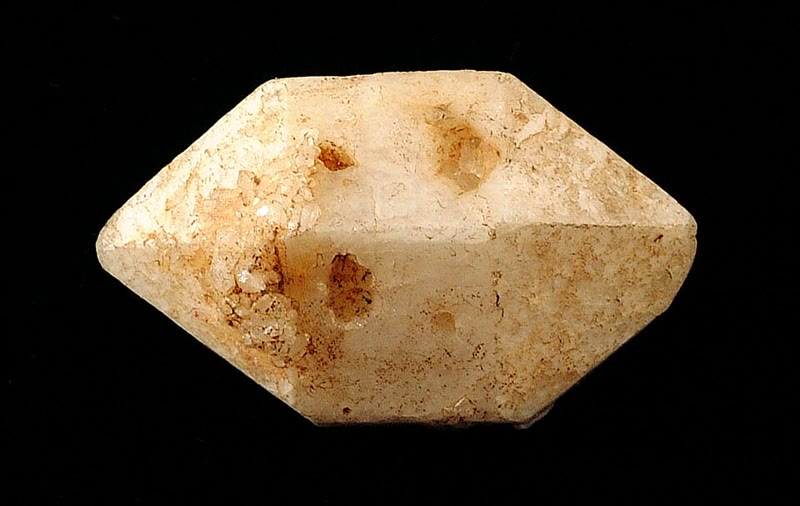
\includegraphics[height=2.75cm]{images/book2/g11-geodil-quartz.jpg}\hfill
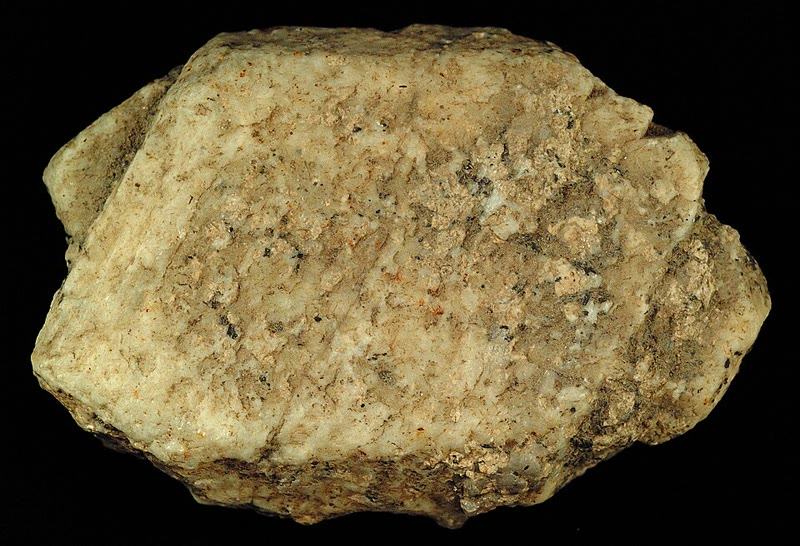
\includegraphics[height=2.75cm]{images/book2/g11-geodil-orthoclase.jpg}\hfill
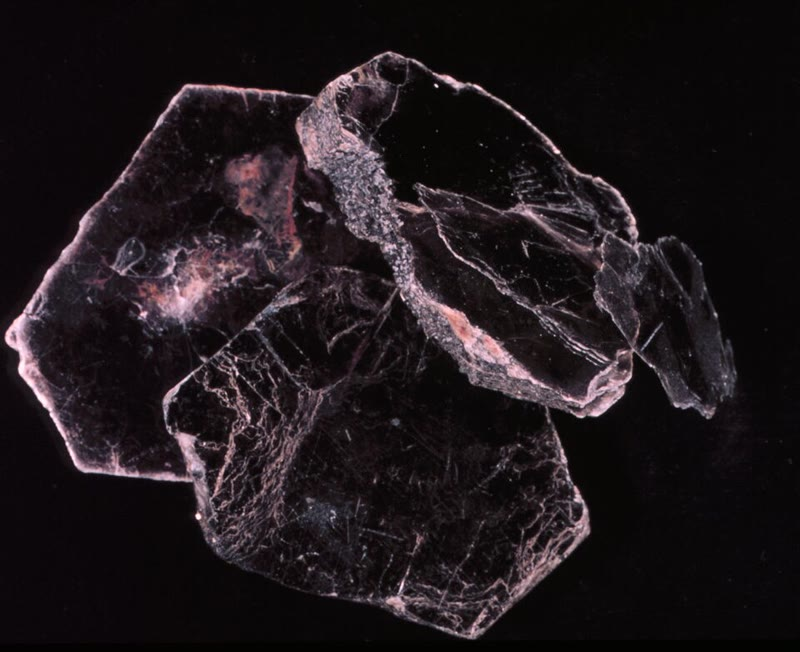
\includegraphics[height=2.75cm]{images/book2/g11-geodil-biotite.jpg}\hfill
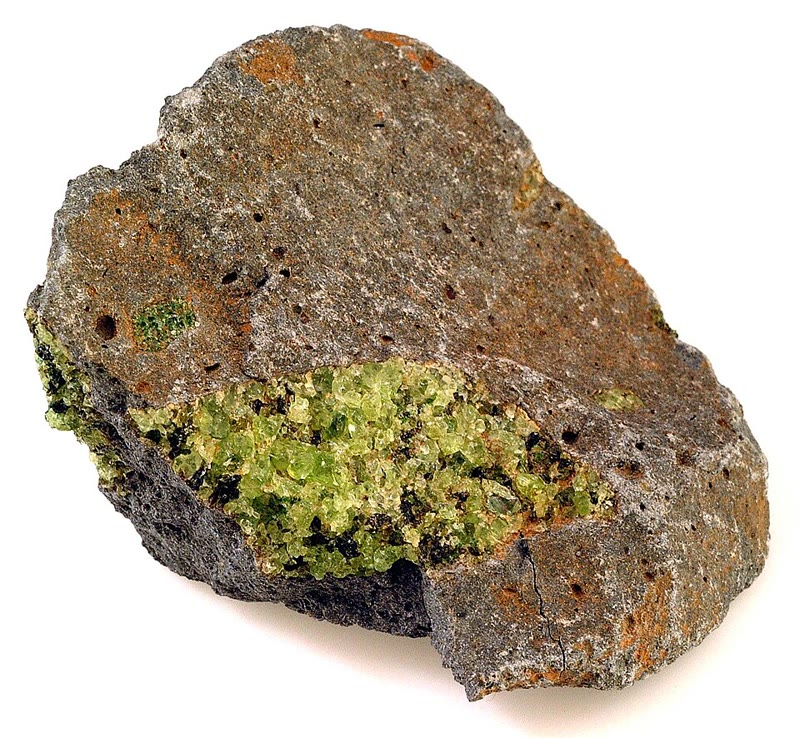
\includegraphics[height=2.75cm]{images/book2/g11-geodil-olivine.jpg}

{\small चट्टान बनाने वाले चार खनिज। बाएँ से दाएँ: क्वार्ट्ज़ का एक क्रिस्टल,
दोनों सिरों पर नुकीला एक षट्भुजीय प्रिज़्म, लगभग \qty{5}{cm} लंबा; एक
ऑर्थोक्लेज़ फ़ेल्डस्पार, साथ बढ़े दो क्रिस्टल, लगभग \qty{7}{cm};
बायोटाइट अभ्रक की षट्भुजीय प्लेटें, लगभग \qty{6}{cm}, जो अपने एकमात्र \omterm{def:g11:minerals:cleavage}{विदलन} के
अनुदिश पतली परतों में फटती हैं; एक बेसाल्ट में ओलिवीन के हरे कण।
फ़ोटो शैनन हाइनल, डार्ला सॉन्ड्रोल, डेक्सटर पर्किन्स और नेसा यूल,
भूविज्ञान डिजिटल छवि पुस्तकालय (CC0)।}
\end{omfigure}
% ledger: photo:g11-quartz, photo:g11-orthoclase, photo:g11-biotite, photo:g11-olivine

\section{सिलिकेट}

\paragraph{दो तत्त्व भूपर्पटी बनाते हैं।} महाद्वीपीय भूपर्पटी का
रासायनिक संघटन बहुत-सी चट्टानों के विश्लेषणों से ज्ञात है, जो
ऑक्साइडों के प्रतिशत के रूप में दिए जाते हैं: लगभग \qty{60.6}{\percent} \ce{SiO2},
\qty{15.9}{\percent} \ce{Al2O3}, इत्यादि। इनसे, और परमाणुओं के
द्रव्यमानों से, हर तत्त्व का द्रव्यमान निकलता है। ऑक्सीजन महाद्वीपीय भूपर्पटी के द्रव्यमान का
\qty{46}{\percent} बनाती है और सिलिकन \qty{28}{\percent}: दो
तत्त्व, द्रव्यमान का लगभग तीन-चौथाई। छह धातुओं --- ऐलुमिनियम,
लोहा, कैल्सियम, मैग्नीशियम, सोडियम और पोटैशियम --- के साथ वे उसका
\qty{99}{\percent} से अधिक बनाते हैं।
% ledger: rg14:crust, ciaaw:O, ciaaw:Si, ciaaw:Al, ciaaw:Fe, ciaaw:Ca, ciaaw:Mg, ciaaw:Na, ciaaw:K, ciaaw:Ti, ciaaw:Mn, ciaaw:P
% values (mineral_density.py): bulk_O 46.36, bulk_Si 28.30, O+Si 74.66, eight elements 99.43

\begin{omfigure}
\begin{tikzpicture}
\begin{axis}[omrecord, width=0.82\linewidth, height=5.6cm, ybar, bar width=14pt,
  ymin=0, ymax=55, xtick=data, enlarge x limits=0.06,
  xticklabels from table={figdata/out/grade-11-mineral_density-elements.dat}{symbol},
  ylabel={द्रव्यमान में अंश (\unit{\percent})},
  nodes near coords, every node near coord/.append style={font=\scriptsize, /pgf/number format/.cd, fixed, precision=1},
  xmajorgrids=false]
% computed in figdata/grade-11/mineral_density.py; ledger: rg14:crust, ciaaw:*
\addplot[fill=omDef!55, draw=omDef] table[x expr=\coordindex, y=frac] {figdata/out/grade-11-mineral_density-elements.dat};
\end{axis}
\end{tikzpicture}

{\small महाद्वीपीय भूपर्पटी के तत्त्व, उसके द्रव्यमान में अंशों के रूप में,
ऑक्साइडों में उसके औसत संघटन से परिकलित (रुडनिक और गाओ, 2014)।
अकेले ऑक्सीजन और सिलिकन द्रव्यमान का लगभग तीन-चौथाई बनाते हैं।}
\end{omfigure}

\paragraph{सिलिकन--ऑक्सीजन चतुष्फलक।} सिलिकन परमाणु छोटा होता है, और
उसके चारों ओर चार ऑक्सीजन परमाणु समा जाते हैं, एक चतुष्फलक के कोनों पर, चार
त्रिभुजाकार फलकों वाला एक पिरामिड। इस समूह में एक सिलिकन आयन \ce{Si^4+} और
चार ऑक्सीजन आयन \ce{O^2-} हैं: इस पर $4 - 4 \times 2 = -4$ का आवेश है,
जिसे दूसरे आयन --- या दूसरे चतुष्फलक --- संतुलित करें।

\begin{definition}[सिलिकेट; सिलिकन--ऑक्सीजन चतुष्फलक]\label{def:g11:minerals:silicate}
\emph{सिलिकन--ऑक्सीजन चतुष्फलक}\index{सिलिकन--ऑक्सीजन चतुष्फलक}
समूह \ce{SiO4} है, जो एक सिलिकन परमाणु और उसके चारों ओर के चार ऑक्सीजन
परमाणुओं से बनता है, एक चतुष्फलक के कोनों पर। \emph{सिलिकेट}\index{सिलिकेट}
सिलिकन--ऑक्सीजन चतुष्फलकों से बना खनिज है, जो अकेले हों या साझा कोनों
द्वारा एक-दूसरे से जुड़े हों।
\end{definition}
% ledger: tulane:silicates

चतुष्फलक ऑक्सीजन साझा करके जुड़ते हैं: एक चतुष्फलक का कोना अगले का
कोना होता है। हर चतुष्फलक कितने कोने साझा करता है, यह
\omterm{def:g11:minerals:silicate}{सिलिकेट} की संरचना, और उसका सूत्र, तय करता है।
\begin{itemize}
  \item \emph{पृथक चतुष्फलक}, जो कोई कोना साझा नहीं करते और अपने बीच के
        धातु आयनों द्वारा जुड़े रहते हैं; उदाहरण के लिए ओलिवीन, \ce{(Mg,Fe)2SiO4}।
  \item \emph{एकल शृंखलाएँ}, हर चतुष्फलक अपने पड़ोसियों के साथ दो कोने
        साझा करता है: पाइरॉक्सीन।
  \item \emph{द्वि-शृंखलाएँ}, दो एकल शृंखलाएँ अगल-बगल जुड़ी हुईं,
        चतुष्फलक बारी-बारी से दो या तीन कोने साझा करते हैं: ऐम्फ़िबोल।
  \item \emph{परतें}, हर चतुष्फलक तीन कोने साझा करता है: अभ्रक,
        और मृदाओं के \omterm{def:g10:soil-formation:clay}{मृत्तिका खनिज} (\cref{ch:g10:soil-formation})।
  \item \emph{ढाँचे}, हर चतुष्फलक चारों कोने साझा करता है, अंतरिक्ष की तीनों
        दिशाओं में: क्वार्ट्ज़, \ce{SiO2}, और --- कुछ सिलिकन के स्थान पर
        ऐलुमिनियम के साथ --- फ़ेल्डस्पार।
\end{itemize}
% ledger: tulane:silicates

\begin{omfigure}
\begin{tikzpicture}[font=\footnotesize]
  % coordinates generated once by a small script (scratch, not kept): kagome net of side 0.62 cm,
  % a regular tetrahedron in perspective, and a framework piece of five tetrahedra (painter's order)
  % (a) one SiO4 tetrahedron, drawn in perspective; the silicon (black) at its centre
  \fill[omDef!12] (2.300,2.979) -- (1.927,1.372) -- (1.221,0.629) -- (3.752,0.820) -- cycle;
  \draw[densely dashed, omDef!60, line width=0.6pt] (2.300,2.979) -- (1.927,1.372);
  \draw[omDef!70!black, line width=0.6pt] (2.300,2.979) -- (1.221,0.629);
  \draw[omDef!70!black, line width=0.6pt] (2.300,2.979) -- (3.752,0.820);
  \draw[densely dashed, omDef!60, line width=0.6pt] (1.927,1.372) -- (1.221,0.629);
  \draw[densely dashed, omDef!60, line width=0.6pt] (1.927,1.372) -- (3.752,0.820);
  \draw[omDef!70!black, line width=0.6pt] (1.221,0.629) -- (3.752,0.820);
  \draw[black!55, line width=0.4pt] (2.300,1.450) -- (2.300,2.979);
  \draw[black!55, line width=0.4pt] (2.300,1.450) -- (1.927,1.372);
  \draw[black!55, line width=0.4pt] (2.300,1.450) -- (1.221,0.629);
  \draw[black!55, line width=0.4pt] (2.300,1.450) -- (3.752,0.820);
  \fill[black] (2.300,1.450) circle (2.2pt);
  \filldraw[fill=omThm!35, draw=omThm!80!black, line width=0.4pt] (2.300,2.979) circle (4.2pt);
  \filldraw[fill=omThm!35, draw=omThm!80!black, line width=0.4pt] (1.927,1.372) circle (4.2pt);
  \filldraw[fill=omThm!35, draw=omThm!80!black, line width=0.4pt] (1.221,0.629) circle (4.2pt);
  \filldraw[fill=omThm!35, draw=omThm!80!black, line width=0.4pt] (3.752,0.820) circle (4.2pt);
  % coordinates for labels: Si 2.300,1.450; apex 2.300,2.979
  % (b) isolated tetrahedra (olivine)
  \filldraw[fill=omDef!22, draw=omDef!70!black, line width=0.5pt] (6.200,0.900) -- (6.820,0.900) -- (6.510,1.437) -- cycle;
  \fill[black] (6.510,1.079) circle (0.9pt);
  \filldraw[fill=omDef!22, draw=omDef!70!black, line width=0.5pt] (8.370,1.437) -- (8.990,1.437) -- (8.680,1.974) -- cycle;
  \fill[black] (8.680,1.616) circle (0.9pt);
  \filldraw[fill=omDef!22, draw=omDef!70!black, line width=0.5pt] (8.060,1.974) -- (7.750,2.511) -- (8.370,2.511) -- cycle;
  \fill[black] (8.060,2.332) circle (0.9pt);
  \filldraw[fill=omDef!22, draw=omDef!70!black, line width=0.5pt] (8.990,0.363) -- (9.610,0.363) -- (9.300,0.900) -- cycle;
  \fill[black] (9.300,0.542) circle (0.9pt);
  \filldraw[fill=omDef!22, draw=omDef!70!black, line width=0.5pt] (9.920,1.974) -- (9.610,2.511) -- (10.230,2.511) -- cycle;
  \fill[black] (9.920,2.332) circle (0.9pt);
  \filldraw[fill=omThm!35, draw=omThm!80!black, line width=0.4pt] (6.200,0.900) circle (1.9pt);
  \filldraw[fill=omThm!35, draw=omThm!80!black, line width=0.4pt] (6.510,1.437) circle (1.9pt);
  \filldraw[fill=omThm!35, draw=omThm!80!black, line width=0.4pt] (6.820,0.900) circle (1.9pt);
  \filldraw[fill=omThm!35, draw=omThm!80!black, line width=0.4pt] (7.750,2.511) circle (1.9pt);
  \filldraw[fill=omThm!35, draw=omThm!80!black, line width=0.4pt] (8.060,1.974) circle (1.9pt);
  \filldraw[fill=omThm!35, draw=omThm!80!black, line width=0.4pt] (8.370,2.511) circle (1.9pt);
  \filldraw[fill=omThm!35, draw=omThm!80!black, line width=0.4pt] (8.370,1.437) circle (1.9pt);
  \filldraw[fill=omThm!35, draw=omThm!80!black, line width=0.4pt] (8.680,1.974) circle (1.9pt);
  \filldraw[fill=omThm!35, draw=omThm!80!black, line width=0.4pt] (8.990,1.437) circle (1.9pt);
  \filldraw[fill=omThm!35, draw=omThm!80!black, line width=0.4pt] (9.610,2.511) circle (1.9pt);
  \filldraw[fill=omThm!35, draw=omThm!80!black, line width=0.4pt] (8.990,0.363) circle (1.9pt);
  \filldraw[fill=omThm!35, draw=omThm!80!black, line width=0.4pt] (9.300,0.900) circle (1.9pt);
  \filldraw[fill=omThm!35, draw=omThm!80!black, line width=0.4pt] (9.920,1.974) circle (1.9pt);
  \filldraw[fill=omThm!35, draw=omThm!80!black, line width=0.4pt] (10.230,2.511) circle (1.9pt);
  \filldraw[fill=omThm!35, draw=omThm!80!black, line width=0.4pt] (9.610,0.363) circle (1.9pt);
  % (c) single chain (pyroxenes)
  \filldraw[fill=omDef!22, draw=omDef!70!black, line width=0.5pt] (11.400,1.600) -- (12.020,1.600) -- (11.710,2.137) -- cycle;
  \fill[black] (11.710,1.779) circle (0.9pt);
  \filldraw[fill=omDef!22, draw=omDef!70!black, line width=0.5pt] (12.330,1.063) -- (12.020,1.600) -- (12.640,1.600) -- cycle;
  \fill[black] (12.330,1.421) circle (0.9pt);
  \filldraw[fill=omDef!22, draw=omDef!70!black, line width=0.5pt] (12.640,1.600) -- (13.260,1.600) -- (12.950,2.137) -- cycle;
  \fill[black] (12.950,1.779) circle (0.9pt);
  \filldraw[fill=omDef!22, draw=omDef!70!black, line width=0.5pt] (13.570,1.063) -- (13.260,1.600) -- (13.880,1.600) -- cycle;
  \fill[black] (13.570,1.421) circle (0.9pt);
  \filldraw[fill=omDef!22, draw=omDef!70!black, line width=0.5pt] (13.880,1.600) -- (14.500,1.600) -- (14.190,2.137) -- cycle;
  \fill[black] (14.190,1.779) circle (0.9pt);
  \filldraw[fill=omDef!22, draw=omDef!70!black, line width=0.5pt] (14.810,1.063) -- (14.500,1.600) -- (15.120,1.600) -- cycle;
  \fill[black] (14.810,1.421) circle (0.9pt);
  \filldraw[fill=omDef!22, draw=omDef!70!black, line width=0.5pt] (15.120,1.600) -- (15.740,1.600) -- (15.430,2.137) -- cycle;
  \fill[black] (15.430,1.779) circle (0.9pt);
  \filldraw[fill=omThm!35, draw=omThm!80!black, line width=0.4pt] (11.400,1.600) circle (1.9pt);
  \filldraw[fill=omThm!35, draw=omThm!80!black, line width=0.4pt] (11.710,2.137) circle (1.9pt);
  \filldraw[fill=omThm!35, draw=omThm!80!black, line width=0.4pt] (12.020,1.600) circle (1.9pt);
  \filldraw[fill=omThm!35, draw=omThm!80!black, line width=0.4pt] (12.330,1.063) circle (1.9pt);
  \filldraw[fill=omThm!35, draw=omThm!80!black, line width=0.4pt] (12.640,1.600) circle (1.9pt);
  \filldraw[fill=omThm!35, draw=omThm!80!black, line width=0.4pt] (12.950,2.137) circle (1.9pt);
  \filldraw[fill=omThm!35, draw=omThm!80!black, line width=0.4pt] (13.260,1.600) circle (1.9pt);
  \filldraw[fill=omThm!35, draw=omThm!80!black, line width=0.4pt] (13.570,1.063) circle (1.9pt);
  \filldraw[fill=omThm!35, draw=omThm!80!black, line width=0.4pt] (13.880,1.600) circle (1.9pt);
  \filldraw[fill=omThm!35, draw=omThm!80!black, line width=0.4pt] (14.190,2.137) circle (1.9pt);
  \filldraw[fill=omThm!35, draw=omThm!80!black, line width=0.4pt] (14.500,1.600) circle (1.9pt);
  \filldraw[fill=omThm!35, draw=omThm!80!black, line width=0.4pt] (14.810,1.063) circle (1.9pt);
  \filldraw[fill=omThm!35, draw=omThm!80!black, line width=0.4pt] (15.120,1.600) circle (1.9pt);
  \filldraw[fill=omThm!35, draw=omThm!80!black, line width=0.4pt] (15.430,2.137) circle (1.9pt);
  \filldraw[fill=omThm!35, draw=omThm!80!black, line width=0.4pt] (15.740,1.600) circle (1.9pt);
  % (d) double chain (amphiboles)
  \filldraw[fill=omDef!22, draw=omDef!70!black, line width=0.5pt] (0.600,-3.550) -- (1.220,-3.550) -- (0.910,-3.013) -- cycle;
  \fill[black] (0.910,-3.371) circle (0.9pt);
  \filldraw[fill=omDef!22, draw=omDef!70!black, line width=0.5pt] (1.530,-4.087) -- (1.220,-3.550) -- (1.840,-3.550) -- cycle;
  \fill[black] (1.530,-3.729) circle (0.9pt);
  \filldraw[fill=omDef!22, draw=omDef!70!black, line width=0.5pt] (1.840,-3.550) -- (2.460,-3.550) -- (2.150,-3.013) -- cycle;
  \fill[black] (2.150,-3.371) circle (0.9pt);
  \filldraw[fill=omDef!22, draw=omDef!70!black, line width=0.5pt] (2.770,-4.087) -- (2.460,-3.550) -- (3.080,-3.550) -- cycle;
  \fill[black] (2.770,-3.729) circle (0.9pt);
  \filldraw[fill=omDef!22, draw=omDef!70!black, line width=0.5pt] (3.080,-3.550) -- (3.700,-3.550) -- (3.390,-3.013) -- cycle;
  \fill[black] (3.390,-3.371) circle (0.9pt);
  \filldraw[fill=omDef!22, draw=omDef!70!black, line width=0.5pt] (4.010,-4.087) -- (3.700,-3.550) -- (4.320,-3.550) -- cycle;
  \fill[black] (4.010,-3.729) circle (0.9pt);
  \filldraw[fill=omDef!22, draw=omDef!70!black, line width=0.5pt] (4.320,-3.550) -- (4.940,-3.550) -- (4.630,-3.013) -- cycle;
  \fill[black] (4.630,-3.371) circle (0.9pt);
  \filldraw[fill=omDef!22, draw=omDef!70!black, line width=0.5pt] (0.910,-3.013) -- (0.600,-2.476) -- (1.220,-2.476) -- cycle;
  \fill[black] (0.910,-2.655) circle (0.9pt);
  \filldraw[fill=omDef!22, draw=omDef!70!black, line width=0.5pt] (1.220,-2.476) -- (1.840,-2.476) -- (1.530,-1.939) -- cycle;
  \fill[black] (1.530,-2.297) circle (0.9pt);
  \filldraw[fill=omDef!22, draw=omDef!70!black, line width=0.5pt] (2.150,-3.013) -- (1.840,-2.476) -- (2.460,-2.476) -- cycle;
  \fill[black] (2.150,-2.655) circle (0.9pt);
  \filldraw[fill=omDef!22, draw=omDef!70!black, line width=0.5pt] (2.460,-2.476) -- (3.080,-2.476) -- (2.770,-1.939) -- cycle;
  \fill[black] (2.770,-2.297) circle (0.9pt);
  \filldraw[fill=omDef!22, draw=omDef!70!black, line width=0.5pt] (3.390,-3.013) -- (3.080,-2.476) -- (3.700,-2.476) -- cycle;
  \fill[black] (3.390,-2.655) circle (0.9pt);
  \filldraw[fill=omDef!22, draw=omDef!70!black, line width=0.5pt] (3.700,-2.476) -- (4.320,-2.476) -- (4.010,-1.939) -- cycle;
  \fill[black] (4.010,-2.297) circle (0.9pt);
  \filldraw[fill=omDef!22, draw=omDef!70!black, line width=0.5pt] (4.630,-3.013) -- (4.320,-2.476) -- (4.940,-2.476) -- cycle;
  \fill[black] (4.630,-2.655) circle (0.9pt);
  \filldraw[fill=omThm!35, draw=omThm!80!black, line width=0.4pt] (0.600,-2.476) circle (1.9pt);
  \filldraw[fill=omThm!35, draw=omThm!80!black, line width=0.4pt] (0.600,-3.550) circle (1.9pt);
  \filldraw[fill=omThm!35, draw=omThm!80!black, line width=0.4pt] (0.910,-3.013) circle (1.9pt);
  \filldraw[fill=omThm!35, draw=omThm!80!black, line width=0.4pt] (1.220,-2.476) circle (1.9pt);
  \filldraw[fill=omThm!35, draw=omThm!80!black, line width=0.4pt] (1.530,-1.939) circle (1.9pt);
  \filldraw[fill=omThm!35, draw=omThm!80!black, line width=0.4pt] (1.220,-3.550) circle (1.9pt);
  \filldraw[fill=omThm!35, draw=omThm!80!black, line width=0.4pt] (1.840,-2.476) circle (1.9pt);
  \filldraw[fill=omThm!35, draw=omThm!80!black, line width=0.4pt] (1.530,-4.087) circle (1.9pt);
  \filldraw[fill=omThm!35, draw=omThm!80!black, line width=0.4pt] (1.840,-3.550) circle (1.9pt);
  \filldraw[fill=omThm!35, draw=omThm!80!black, line width=0.4pt] (2.150,-3.013) circle (1.9pt);
  \filldraw[fill=omThm!35, draw=omThm!80!black, line width=0.4pt] (2.460,-2.476) circle (1.9pt);
  \filldraw[fill=omThm!35, draw=omThm!80!black, line width=0.4pt] (2.770,-1.939) circle (1.9pt);
  \filldraw[fill=omThm!35, draw=omThm!80!black, line width=0.4pt] (2.460,-3.550) circle (1.9pt);
  \filldraw[fill=omThm!35, draw=omThm!80!black, line width=0.4pt] (3.080,-2.476) circle (1.9pt);
  \filldraw[fill=omThm!35, draw=omThm!80!black, line width=0.4pt] (2.770,-4.087) circle (1.9pt);
  \filldraw[fill=omThm!35, draw=omThm!80!black, line width=0.4pt] (3.080,-3.550) circle (1.9pt);
  \filldraw[fill=omThm!35, draw=omThm!80!black, line width=0.4pt] (3.390,-3.013) circle (1.9pt);
  \filldraw[fill=omThm!35, draw=omThm!80!black, line width=0.4pt] (3.700,-2.476) circle (1.9pt);
  \filldraw[fill=omThm!35, draw=omThm!80!black, line width=0.4pt] (4.010,-1.939) circle (1.9pt);
  \filldraw[fill=omThm!35, draw=omThm!80!black, line width=0.4pt] (3.700,-3.550) circle (1.9pt);
  \filldraw[fill=omThm!35, draw=omThm!80!black, line width=0.4pt] (4.320,-2.476) circle (1.9pt);
  \filldraw[fill=omThm!35, draw=omThm!80!black, line width=0.4pt] (4.010,-4.087) circle (1.9pt);
  \filldraw[fill=omThm!35, draw=omThm!80!black, line width=0.4pt] (4.320,-3.550) circle (1.9pt);
  \filldraw[fill=omThm!35, draw=omThm!80!black, line width=0.4pt] (4.630,-3.013) circle (1.9pt);
  \filldraw[fill=omThm!35, draw=omThm!80!black, line width=0.4pt] (4.940,-2.476) circle (1.9pt);
  \filldraw[fill=omThm!35, draw=omThm!80!black, line width=0.4pt] (4.940,-3.550) circle (1.9pt);
  % (e) sheet (micas)
  \filldraw[fill=omDef!22, draw=omDef!70!black, line width=0.5pt] (5.900,-4.100) -- (6.520,-4.100) -- (6.210,-3.563) -- cycle;
  \fill[black] (6.210,-3.921) circle (0.9pt);
  \filldraw[fill=omDef!22, draw=omDef!70!black, line width=0.5pt] (7.140,-4.100) -- (7.760,-4.100) -- (7.450,-3.563) -- cycle;
  \fill[black] (7.450,-3.921) circle (0.9pt);
  \filldraw[fill=omDef!22, draw=omDef!70!black, line width=0.5pt] (8.380,-4.100) -- (9.000,-4.100) -- (8.690,-3.563) -- cycle;
  \fill[black] (8.690,-3.921) circle (0.9pt);
  \filldraw[fill=omDef!22, draw=omDef!70!black, line width=0.5pt] (9.620,-4.100) -- (10.240,-4.100) -- (9.930,-3.563) -- cycle;
  \fill[black] (9.930,-3.921) circle (0.9pt);
  \filldraw[fill=omDef!22, draw=omDef!70!black, line width=0.5pt] (6.210,-3.563) -- (5.900,-3.026) -- (6.520,-3.026) -- cycle;
  \fill[black] (6.210,-3.205) circle (0.9pt);
  \filldraw[fill=omDef!22, draw=omDef!70!black, line width=0.5pt] (7.450,-3.563) -- (7.140,-3.026) -- (7.760,-3.026) -- cycle;
  \fill[black] (7.450,-3.205) circle (0.9pt);
  \filldraw[fill=omDef!22, draw=omDef!70!black, line width=0.5pt] (8.690,-3.563) -- (8.380,-3.026) -- (9.000,-3.026) -- cycle;
  \fill[black] (8.690,-3.205) circle (0.9pt);
  \filldraw[fill=omDef!22, draw=omDef!70!black, line width=0.5pt] (9.930,-3.563) -- (9.620,-3.026) -- (10.240,-3.026) -- cycle;
  \fill[black] (9.930,-3.205) circle (0.9pt);
  \filldraw[fill=omDef!22, draw=omDef!70!black, line width=0.5pt] (6.520,-3.026) -- (7.140,-3.026) -- (6.830,-2.489) -- cycle;
  \fill[black] (6.830,-2.847) circle (0.9pt);
  \filldraw[fill=omDef!22, draw=omDef!70!black, line width=0.5pt] (7.760,-3.026) -- (8.380,-3.026) -- (8.070,-2.489) -- cycle;
  \fill[black] (8.070,-2.847) circle (0.9pt);
  \filldraw[fill=omDef!22, draw=omDef!70!black, line width=0.5pt] (9.000,-3.026) -- (9.620,-3.026) -- (9.310,-2.489) -- cycle;
  \fill[black] (9.310,-2.847) circle (0.9pt);
  \filldraw[fill=omDef!22, draw=omDef!70!black, line width=0.5pt] (6.830,-2.489) -- (6.520,-1.952) -- (7.140,-1.952) -- cycle;
  \fill[black] (6.830,-2.131) circle (0.9pt);
  \filldraw[fill=omDef!22, draw=omDef!70!black, line width=0.5pt] (8.070,-2.489) -- (7.760,-1.952) -- (8.380,-1.952) -- cycle;
  \fill[black] (8.070,-2.131) circle (0.9pt);
  \filldraw[fill=omDef!22, draw=omDef!70!black, line width=0.5pt] (9.310,-2.489) -- (9.000,-1.952) -- (9.620,-1.952) -- cycle;
  \fill[black] (9.310,-2.131) circle (0.9pt);
  \filldraw[fill=omDef!22, draw=omDef!70!black, line width=0.5pt] (5.900,-1.952) -- (6.520,-1.952) -- (6.210,-1.415) -- cycle;
  \fill[black] (6.210,-1.773) circle (0.9pt);
  \filldraw[fill=omDef!22, draw=omDef!70!black, line width=0.5pt] (7.140,-1.952) -- (7.760,-1.952) -- (7.450,-1.415) -- cycle;
  \fill[black] (7.450,-1.773) circle (0.9pt);
  \filldraw[fill=omDef!22, draw=omDef!70!black, line width=0.5pt] (8.380,-1.952) -- (9.000,-1.952) -- (8.690,-1.415) -- cycle;
  \fill[black] (8.690,-1.773) circle (0.9pt);
  \filldraw[fill=omDef!22, draw=omDef!70!black, line width=0.5pt] (9.620,-1.952) -- (10.240,-1.952) -- (9.930,-1.415) -- cycle;
  \fill[black] (9.930,-1.773) circle (0.9pt);
  \filldraw[fill=omThm!35, draw=omThm!80!black, line width=0.4pt] (5.900,-1.952) circle (1.9pt);
  \filldraw[fill=omThm!35, draw=omThm!80!black, line width=0.4pt] (6.210,-1.415) circle (1.9pt);
  \filldraw[fill=omThm!35, draw=omThm!80!black, line width=0.4pt] (5.900,-3.026) circle (1.9pt);
  \filldraw[fill=omThm!35, draw=omThm!80!black, line width=0.4pt] (6.520,-1.952) circle (1.9pt);
  \filldraw[fill=omThm!35, draw=omThm!80!black, line width=0.4pt] (5.900,-4.100) circle (1.9pt);
  \filldraw[fill=omThm!35, draw=omThm!80!black, line width=0.4pt] (6.210,-3.563) circle (1.9pt);
  \filldraw[fill=omThm!35, draw=omThm!80!black, line width=0.4pt] (6.520,-3.026) circle (1.9pt);
  \filldraw[fill=omThm!35, draw=omThm!80!black, line width=0.4pt] (6.830,-2.489) circle (1.9pt);
  \filldraw[fill=omThm!35, draw=omThm!80!black, line width=0.4pt] (7.140,-1.952) circle (1.9pt);
  \filldraw[fill=omThm!35, draw=omThm!80!black, line width=0.4pt] (7.450,-1.415) circle (1.9pt);
  \filldraw[fill=omThm!35, draw=omThm!80!black, line width=0.4pt] (6.520,-4.100) circle (1.9pt);
  \filldraw[fill=omThm!35, draw=omThm!80!black, line width=0.4pt] (7.140,-3.026) circle (1.9pt);
  \filldraw[fill=omThm!35, draw=omThm!80!black, line width=0.4pt] (7.760,-1.952) circle (1.9pt);
  \filldraw[fill=omThm!35, draw=omThm!80!black, line width=0.4pt] (7.140,-4.100) circle (1.9pt);
  \filldraw[fill=omThm!35, draw=omThm!80!black, line width=0.4pt] (7.450,-3.563) circle (1.9pt);
  \filldraw[fill=omThm!35, draw=omThm!80!black, line width=0.4pt] (7.760,-3.026) circle (1.9pt);
  \filldraw[fill=omThm!35, draw=omThm!80!black, line width=0.4pt] (8.070,-2.489) circle (1.9pt);
  \filldraw[fill=omThm!35, draw=omThm!80!black, line width=0.4pt] (8.380,-1.952) circle (1.9pt);
  \filldraw[fill=omThm!35, draw=omThm!80!black, line width=0.4pt] (8.690,-1.415) circle (1.9pt);
  \filldraw[fill=omThm!35, draw=omThm!80!black, line width=0.4pt] (7.760,-4.100) circle (1.9pt);
  \filldraw[fill=omThm!35, draw=omThm!80!black, line width=0.4pt] (8.380,-3.026) circle (1.9pt);
  \filldraw[fill=omThm!35, draw=omThm!80!black, line width=0.4pt] (9.000,-1.952) circle (1.9pt);
  \filldraw[fill=omThm!35, draw=omThm!80!black, line width=0.4pt] (8.380,-4.100) circle (1.9pt);
  \filldraw[fill=omThm!35, draw=omThm!80!black, line width=0.4pt] (8.690,-3.563) circle (1.9pt);
  \filldraw[fill=omThm!35, draw=omThm!80!black, line width=0.4pt] (9.000,-3.026) circle (1.9pt);
  \filldraw[fill=omThm!35, draw=omThm!80!black, line width=0.4pt] (9.310,-2.489) circle (1.9pt);
  \filldraw[fill=omThm!35, draw=omThm!80!black, line width=0.4pt] (9.620,-1.952) circle (1.9pt);
  \filldraw[fill=omThm!35, draw=omThm!80!black, line width=0.4pt] (9.930,-1.415) circle (1.9pt);
  \filldraw[fill=omThm!35, draw=omThm!80!black, line width=0.4pt] (9.000,-4.100) circle (1.9pt);
  \filldraw[fill=omThm!35, draw=omThm!80!black, line width=0.4pt] (9.620,-3.026) circle (1.9pt);
  \filldraw[fill=omThm!35, draw=omThm!80!black, line width=0.4pt] (10.240,-1.952) circle (1.9pt);
  \filldraw[fill=omThm!35, draw=omThm!80!black, line width=0.4pt] (9.620,-4.100) circle (1.9pt);
  \filldraw[fill=omThm!35, draw=omThm!80!black, line width=0.4pt] (9.930,-3.563) circle (1.9pt);
  \filldraw[fill=omThm!35, draw=omThm!80!black, line width=0.4pt] (10.240,-3.026) circle (1.9pt);
  \filldraw[fill=omThm!35, draw=omThm!80!black, line width=0.4pt] (10.240,-4.100) circle (1.9pt);
  % (f) framework: a tetrahedron sharing all four corners
  \filldraw[fill=omThm!35, draw=omThm!80!black, line width=0.4pt] (12.990,-1.963) circle (2.1pt);
  \filldraw[fill=omThm!35, draw=omThm!80!black, line width=0.4pt] (12.896,-3.062) circle (2.1pt);
  \filldraw[fill=omDef!14, draw=omDef!70!black, line width=0.45pt, fill opacity=0.85] (12.896,-3.062) -- (12.990,-1.963) -- (12.299,-2.380) -- cycle;
  \filldraw[fill=omThm!35, draw=omThm!80!black, line width=0.4pt] (15.186,-2.119) circle (2.1pt);
  \filldraw[fill=omDef!14, draw=omDef!70!black, line width=0.45pt, fill opacity=0.85] (12.896,-3.062) -- (13.398,-2.458) -- (12.990,-1.963) -- cycle;
  \filldraw[fill=omThm!35, draw=omThm!80!black, line width=0.4pt] (15.092,-3.219) circle (2.1pt);
  \fill[black] (12.896,-2.466) circle (1.1pt);
  \filldraw[fill=omDef!34, draw=omDef!70!black, line width=0.45pt, fill opacity=0.85] (13.398,-2.458) -- (12.990,-1.963) -- (12.299,-2.380) -- cycle;
  \filldraw[fill=omDef!14, draw=omDef!70!black, line width=0.45pt, fill opacity=0.85] (15.092,-3.219) -- (15.186,-2.119) -- (14.496,-2.536) -- cycle;
  \filldraw[fill=omDef!25, draw=omDef!70!black, line width=0.45pt, fill opacity=0.85] (12.896,-3.062) -- (12.299,-2.380) -- (13.398,-2.458) -- cycle;
  \filldraw[fill=omDef!14, draw=omDef!70!black, line width=0.45pt, fill opacity=0.85] (15.092,-3.219) -- (15.595,-2.614) -- (15.186,-2.119) -- cycle;
  \fill[black] (15.092,-2.622) circle (1.1pt);
  \filldraw[fill=omThm!35, draw=omThm!80!black, line width=0.4pt] (12.299,-2.380) circle (2.1pt);
  \filldraw[fill=omDef!34, draw=omDef!70!black, line width=0.45pt, fill opacity=0.85] (15.595,-2.614) -- (15.186,-2.119) -- (14.496,-2.536) -- cycle;
  \filldraw[fill=omDef!25, draw=omDef!70!black, line width=0.45pt, fill opacity=0.85] (15.092,-3.219) -- (14.496,-2.536) -- (15.595,-2.614) -- cycle;
  \filldraw[fill=omThm!35, draw=omThm!80!black, line width=0.4pt] (13.398,-2.458) circle (2.1pt);
  \filldraw[fill=omThm!35, draw=omThm!80!black, line width=0.4pt] (14.496,-2.536) circle (2.1pt);
  \filldraw[fill=omDef!14, draw=omDef!70!black, line width=0.45pt, fill opacity=0.85] (13.900,-1.853) -- (14.496,-2.536) -- (13.398,-2.458) -- cycle;
  \filldraw[fill=omThm!35, draw=omThm!80!black, line width=0.4pt] (15.595,-2.614) circle (2.1pt);
  \filldraw[fill=omDef!14, draw=omDef!70!black, line width=0.45pt, fill opacity=0.85] (13.398,-2.458) -- (13.806,-2.953) -- (14.496,-2.536) -- cycle;
  \fill[black] (13.900,-2.450) circle (1.1pt);
  \filldraw[fill=omDef!22, draw=omDef!70!black, line width=0.45pt, fill opacity=0.85] (13.900,-1.853) -- (13.398,-2.458) -- (13.806,-2.953) -- cycle;
  \filldraw[fill=omDef!37, draw=omDef!70!black, line width=0.45pt, fill opacity=0.85] (13.900,-1.853) -- (13.806,-2.953) -- (14.496,-2.536) -- cycle;
  \filldraw[fill=omThm!35, draw=omThm!80!black, line width=0.4pt] (13.994,-0.754) circle (2.1pt);
  \filldraw[fill=omThm!35, draw=omThm!80!black, line width=0.4pt] (13.900,-1.853) circle (2.1pt);
  \filldraw[fill=omThm!35, draw=omThm!80!black, line width=0.4pt] (13.806,-2.953) circle (2.1pt);
  \filldraw[fill=omDef!14, draw=omDef!70!black, line width=0.45pt, fill opacity=0.85] (13.900,-1.853) -- (13.994,-0.754) -- (13.304,-1.171) -- cycle;
  \filldraw[fill=omDef!14, draw=omDef!70!black, line width=0.45pt, fill opacity=0.85] (13.900,-1.853) -- (14.402,-1.249) -- (13.994,-0.754) -- cycle;
  \filldraw[fill=omThm!35, draw=omThm!80!black, line width=0.4pt] (13.712,-4.053) circle (2.1pt);
  \fill[black] (13.900,-1.256) circle (1.1pt);
  \filldraw[fill=omDef!14, draw=omDef!70!black, line width=0.45pt, fill opacity=0.85] (13.712,-4.053) -- (13.806,-2.953) -- (13.116,-3.370) -- cycle;
  \filldraw[fill=omDef!34, draw=omDef!70!black, line width=0.45pt, fill opacity=0.85] (14.402,-1.249) -- (13.994,-0.754) -- (13.304,-1.171) -- cycle;
  \filldraw[fill=omDef!14, draw=omDef!70!black, line width=0.45pt, fill opacity=0.85] (13.712,-4.053) -- (14.214,-3.448) -- (13.806,-2.953) -- cycle;
  \filldraw[fill=omDef!25, draw=omDef!70!black, line width=0.45pt, fill opacity=0.85] (13.900,-1.853) -- (13.304,-1.171) -- (14.402,-1.249) -- cycle;
  \fill[black] (13.712,-3.456) circle (1.1pt);
  \filldraw[fill=omThm!35, draw=omThm!80!black, line width=0.4pt] (13.304,-1.171) circle (2.1pt);
  \filldraw[fill=omDef!34, draw=omDef!70!black, line width=0.45pt, fill opacity=0.85] (14.214,-3.448) -- (13.806,-2.953) -- (13.116,-3.370) -- cycle;
  \filldraw[fill=omDef!25, draw=omDef!70!black, line width=0.45pt, fill opacity=0.85] (13.712,-4.053) -- (13.116,-3.370) -- (14.214,-3.448) -- cycle;
  \filldraw[fill=omThm!35, draw=omThm!80!black, line width=0.4pt] (14.402,-1.249) circle (2.1pt);
  \filldraw[fill=omThm!35, draw=omThm!80!black, line width=0.4pt] (13.116,-3.370) circle (2.1pt);
  \filldraw[fill=omThm!35, draw=omThm!80!black, line width=0.4pt] (14.214,-3.448) circle (2.1pt);
  % labels
  \draw[black!60] (2.30,2.98) -- (3.35,3.25); \node[anchor=west] at (3.35,3.25) {ऑक्सीजन};
  \draw[black!60] (2.30,1.45) -- (3.55,2.15); \node[anchor=west] at (3.55,2.15) {सिलिकन};
  \node[align=center] at (2.3,-0.15) {(a) एक चतुष्फलक, \ce{SiO4}};
  \node[align=center] at (8.2,-0.15) {(b) पृथक चतुष्फलक:\\ओलिवीन};
  \node[align=center] at (13.5,-0.15) {(c) एकल शृंखला:\\पाइरॉक्सीन};
  \node[align=center] at (2.75,-4.85) {(d) द्वि-शृंखला:\\ऐम्फ़िबोल};
  \node[align=center] at (8.1,-4.85) {(e) परत:\\अभ्रक};
  \node[align=center] at (13.9,-4.85) {(f) ढाँचा:\\क्वार्ट्ज़, फ़ेल्डस्पार};
\end{tikzpicture}

{\small (a) \omterm{def:g11:minerals:silicate}{सिलिकन--ऑक्सीजन चतुष्फलक}: एक सिलिकन परमाणु (काला) और एक चतुष्फलक के
कोनों पर चार ऑक्सीजन परमाणु (गुलाबी)। (b)--(e) ऊपर से देखे गए
चतुष्फलक, हर एक त्रिभुज के रूप में: वृत्त उसके आधार के ऑक्सीजन हैं,
बिंदु सिलिकन, चौथे ऑक्सीजन के नीचे; किसी कोने पर मिलने वाले दो त्रिभुज
वह ऑक्सीजन साझा करते हैं। (f) ढाँचे में हर कोना साझा होता है, तीन
आयामों में: यहाँ एक चतुष्फलक और उसके चार पड़ोसी। चित्र, पैमाने पर
नहीं।}
\end{omfigure}
% ledger: tulane:silicates

\begin{proposition}[ऑक्सीजनों की गिनती]\label{prop:g11:minerals:sharing}
ऐसे \omterm{def:g11:minerals:silicate}{सिलिकेट} में जहाँ हर चतुष्फलक अपने $n$ कोने दूसरे चतुष्फलकों के साथ साझा
करता है, हर सिलिकन परमाणु के लिए $4 - n/2$ ऑक्सीजन परमाणु होते हैं। पृथक
चतुष्फलक \ce{SiO4} देते हैं, एकल शृंखलाएँ \ce{SiO3}, परतें \ce{Si2O5} और
ढाँचे \ce{SiO2}।
\end{proposition}

\begin{proof}
हर चतुष्फलक में एक सिलिकन और चार कोने हैं। जो कोना
साझा नहीं है, वह केवल इसी चतुष्फलक का है और एक ऑक्सीजन गिना जाता है; साझा
कोना दो चतुष्फलकों का है और हर एक में आधा ऑक्सीजन गिना जाता है।
$n$ साझा कोनों के साथ, एक चतुष्फलक के $(4 - n) + n/2 = 4 - n/2$ ऑक्सीजन होते हैं।
$n = 0$, $2$, $3$ और $4$ के लिए यह प्रति सिलिकन $4$, $3$, $5/2$ और $2$ ऑक्सीजन
देता है: \ce{SiO4}, \ce{SiO3}, \ce{Si2O5} और \ce{SiO2}।
\end{proof}

खनिजों के सूत्र इसकी पुष्टि करते हैं। पाइरॉक्सीन ऑजाइट में
\ce{(Si,Al)2O6} है, यानी दो बार \ce{SiO3}, और अभ्रक बायोटाइट में \ce{AlSi3O10},
दस ऑक्सीजनों के लिए चार चतुष्फलक, दो बार \ce{Si2O5}; फ़ेल्डस्पार में चार
चतुष्फलकों में आठ ऑक्सीजन होते हैं, चार बार \ce{SiO2}, ठीक क्वार्ट्ज़ की तरह।
पर आवेश भिन्न होते हैं। क्वार्ट्ज़ उदासीन है: ढाँचे में हर ऑक्सीजन
साझा है, और सिलिकन और ऑक्सीजन के आवेश संतुलित होते हैं। दूसरी
संरचनाओं में असाझा ऑक्सीजन अतिरिक्त ऋणात्मक आवेश ढोते हैं, जिन्हें
धातु आयन संतुलित करते हैं --- ओलिवीन में मैग्नीशियम और लोहा, ऑर्थोक्लेज़ में पोटैशियम, जहाँ
एक ऐलुमिनियम आयन \ce{Al^3+}, सिलिकन आयन \ce{Si^4+} के स्थान पर, एक
आवेश संतुलित करने को छोड़ देता है।
% ledger: wm:densities (formulas)

\begin{definition}[शैलकारी सिलिकेट]\label{def:g11:minerals:rock-forming}
\emph{शैलकारी सिलिकेट}\index{शैलकारी सिलिकेट} \omterm{def:g11:minerals:silicate}{सिलिकेट} खनिजों के वे छह
समूह हैं जो अधिकांश सामान्य आग्नेय और
कायांतरित चट्टानें बनाते हैं: ओलिवीन, पाइरॉक्सीन, ऐम्फ़िबोल, अभ्रक,
फ़ेल्डस्पार और क्वार्ट्ज़। फ़ेल्डस्पार दो प्रकार के होते हैं: \emph{पोटैशियम
फ़ेल्डस्पार}, जैसे ऑर्थोक्लेज़, और \emph{प्लेजियोक्लेज़}, सोडियम और कैल्सियम
वाले फ़ेल्डस्पारों की एक श्रेणी।
\end{definition}
% ledger: tulane:silicates, wm:densities

\begin{center}
\small
\renewcommand{\arraystretch}{1.25}
\begin{tabular}{|l|l|l|c|}
\hline
\textbf{समूह (उदाहरण)} & \textbf{संरचना} & \textbf{सूत्र} & \textbf{घनत्व} \\
 & & & (\unit{g/cm^3}) \\
\hline
ओलिवीन & पृथक चतुष्फलक & \ce{(Mg,Fe)2SiO4} & 3.32 \\
पाइरॉक्सीन (ऑजाइट) & एकल शृंखलाएँ & \ce{(Ca,Na)(Mg,Fe,Al,Ti)(Si,Al)2O6} & 3.4 \\
ऐम्फ़िबोल (हॉर्नब्लेंड) & द्वि-शृंखलाएँ & \ce{Ca2[Mg4(Al,Fe)]Si7AlO22(OH)2} & 3.23 \\
अभ्रक (बायोटाइट) & परतें & \ce{K(Mg,Fe)3AlSi3O10(OH,F)2} & 3.09 \\
अभ्रक (मस्कोवाइट) & परतें & \ce{KAl2(Si3Al)O10(OH,F)2} & 2.82 \\
पोटैशियम फ़ेल्डस्पार (ऑर्थोक्लेज़) & ढाँचा & \ce{KAlSi3O8} & 2.56 \\
प्लेजियोक्लेज़ (ऑलिगोक्लेज़) & ढाँचा & \ce{(Na,Ca)(Si,Al)4O8} & 2.65 \\
क्वार्ट्ज़ & ढाँचा & \ce{SiO2} & 2.62 \\
\hline
\end{tabular}

\smallskip
{\footnotesize \omterm{def:g11:minerals:rock-forming}{शैलकारी सिलिकेट}। सूत्र और माध्य घनत्व
webmineral.com से; कोष्ठक में दो तत्त्वों के बीच का अल्पविराम बताता है कि क्रिस्टल में
उस स्थान को दोनों में से कोई भी ले सकता है।}
\end{center}
% ledger: wm:densities, tulane:silicates

यह तालिका एक ऐसा नियम समेटे है जो इस पुस्तक के शेष भाग में चलता है। पृथक
चतुष्फलकों और शृंखलाओं वाले खनिज, लोहे और मैग्नीशियम से समृद्ध, सबसे
घने हैं, \qty{3.2}{g/cm^3} से ऊपर; ढाँचे, जो सिलिकन, ऐलुमिनियम,
सोडियम, पोटैशियम और कैल्सियम से बने हैं, सबसे हल्के हैं, लगभग \qty{2.6}{g/cm^3}।
अभ्रक बीच में हैं। ओलिवीन और पाइरॉक्सीन प्रावार का \omterm{def:g11:ocean-ridges:peridotite}{पेरिडोटाइट} बनाते हैं;
फ़ेल्डस्पार और क्वार्ट्ज़, महाद्वीपों का ग्रेनाइट: हल्की चट्टान घनी चट्टान
पर तैरती है।
% ledger: wm:densities

\section{खनिज चट्टानें बनाते हैं}

किसी चट्टान का वर्णन सबसे पहले उसके खनिजों और उनके अनुपातों से होता है। पहले के
अध्यायों में मिली तीन चट्टानें इस परास को दिखाती हैं:
\begin{itemize}
  \item \emph{ग्रेनाइट}: क्वार्ट्ज़, पोटैशियम फ़ेल्डस्पार और प्लेजियोक्लेज़, थोड़े
        बायोटाइट या मस्कोवाइट के साथ --- महाद्वीपों की चट्टान;
  \item \emph{बेसाल्ट} और \emph{\omterm{def:g11:ocean-ridges:gabbro}{गैब्रो}}: प्लेजियोक्लेज़ और पाइरॉक्सीन, अक्सर
        ओलिवीन के साथ --- \omterm{def:g11:ocean-ridges:oceanic-lithosphere}{महासागरीय भूपर्पटी} की चट्टानें, पहली बारीक
        कणों वाली, दूसरी मोटे कणों वाली (\cref{ch:g11:igneous-rocks});
  \item \emph{\omterm{def:g11:ocean-ridges:peridotite}{पेरिडोटाइट}}: ज़्यादातर ओलिवीन, पाइरॉक्सीन के साथ --- प्रावार की
        चट्टान।
\end{itemize}
% ledger: nps:granite-minerals, photo:g11-basalt-thin-section, photo:g11-olivine

\begin{omfigure}
\begin{tikzpicture}
\begin{axis}[omrecord, width=0.8\linewidth, height=6.4cm, xbar, bar width=8pt,
  xmin=2.4, xmax=3.5, ymin=-0.7, ymax=8.7, ytick={0,...,8},
  yticklabels={ऑर्थोक्लेज़, क्वार्ट्ज़, ऑलिगोक्लेज़, लैब्राडोराइट, मस्कोवाइट, बायोटाइट, हॉर्नब्लेंड, ओलिवीन, ऑजाइट},
  xlabel={घनत्व (\unit{g/cm^3})}, ymajorgrids=false, clip=false]
% computed in figdata/grade-11/mineral_density.py (density_order); ledger: wm:densities
\addplot[fill=omDef!45, draw=omDef] table[x=rho, y=idx] {figdata/out/grade-11-mineral_density-densities.dat};
\draw[omProp, line width=1pt, dashed] (axis cs:2.6427,-0.7) -- (axis cs:2.6427,8.7) node[above, text height=1.6ex, text depth=0.3ex, font=\scriptsize, text=omProp!80!black] {ग्रेनाइट};
\draw[omThm, line width=1pt, dashed] (axis cs:3.0015,-0.7) -- (axis cs:3.0015,8.7) node[above, text height=1.6ex, text depth=0.3ex, font=\scriptsize, text=omThm] {बेसाल्ट};
\draw[black!70, line width=1pt, dashed] (axis cs:3.34,-0.7) -- (axis cs:3.34,8.7) node[above, font=\scriptsize] {पेरिडोटाइट};
\end{axis}
\end{tikzpicture}

{\small नौ शैलकारी खनिजों के माध्य घनत्व (webmineral.com),
और इस खंड की तीन उदाहरण चट्टानों के घनत्व, नीचे के प्रस्ताव से
परिकलित (धराशायी रेखाएँ): क्वार्ट्ज़, फ़ेल्डस्पारों और
अभ्रकों का एक ग्रेनाइट, प्लेजियोक्लेज़, पाइरॉक्सीन और थोड़े ओलिवीन का एक बेसाल्ट,
ओलिवीन और पाइरॉक्सीन का एक \omterm{def:g11:ocean-ridges:peridotite}{पेरिडोटाइट}।}
\end{omfigure}
% values (mineral_density.py): rho_granite 2.6427, rho_basalt 3.0015, rho_peridotite 3.34

किसी चट्टान का घनत्व उसके खनिजों से निकलता है। चट्टान के एक खंड की कल्पना कीजिए, जिसका
आयतन $V$ है, जिसका अंश $\phi_1$ पहले खनिज से बना है, $\phi_2$
दूसरे से, इत्यादि।

\begin{proposition}[खनिजों से चट्टान का घनत्व]\label{prop:g11:minerals:density}
बिना रंध्रों की चट्टान, जो घनत्व $\rho_1, \rho_2, \dots,
\rho_k$ वाले खनिजों से बनी है जो उसके आयतन के अंश $\phi_1, \phi_2, \dots, \phi_k$ घेरते हैं
($\phi_1 + \dots + \phi_k = 1$), का घनत्व यह होता है:
\[
  \rho = \phi_1 \rho_1 + \phi_2 \rho_2 + \dots + \phi_k \rho_k ,
\]
जो उसके खनिजों के घनत्वों का माध्य है, उनके आयतन-अंशों से
भारित।
\end{proposition}

\begin{proof}
चट्टान के आयतन $V$ में खनिज $i$ आयतन $\phi_i V$ घेरता है और उसका
द्रव्यमान $\rho_i \phi_i V$ है। रंध्र न हों तो चट्टान का द्रव्यमान इन
द्रव्यमानों का योग है, $m = (\phi_1 \rho_1 + \dots + \phi_k \rho_k)\,V$, और उसका
घनत्व $m/V$ है।
\end{proof}

आयतन-अंश कैसे मापे जाते हैं? चट्टान के किसी समतल कटे फलक पर, या किसी
\omterm{def:g11:minerals:thin-section}{पतली काट} (अगला खंड) पर, बिंदुओं का एक नियमित जाल बिछाया जाता है, और
हर बिंदु पर उसके नीचे का खनिज दर्ज किया जाता है। जब कण बिना किसी क्रम
के बिखरे हों, तो किसी खनिज पर पड़ने वाले बिंदुओं का अंश
उसके द्वारा ढके क्षेत्रफल के अंश का अनुमान देता है, और वही उसके द्वारा भरे
आयतन का अंश भी है: एक पतली फाँक पूरे खंड का उचित नमूना है। यह
\emph{बिंदु-गणना} है।

\begin{example}[क्वार्ट्ज़ और पोटैशियम फ़ेल्डस्पार से समृद्ध एक हल्का ग्रेनाइट]
बिंदु-गणना \qty{35}{\percent} क्वार्ट्ज़ (\qty{2.62}{g/cm^3}),
\qty{50}{\percent} ऑर्थोक्लेज़ (\qty{2.56}{g/cm^3}) और \qty{15}{\percent}
ऑलिगोक्लेज़ (\qty{2.65}{g/cm^3}) देती है। चट्टान का घनत्व यह है:
\[
  \rho = 0.35 \times 2.62 + 0.50 \times 2.56 + 0.15 \times 2.65
       = 0.917 + 1.280 + 0.398 \approx \qty{2.59}{g/cm^3}.
\]
मापन परिमाण की इस कोटि की पुष्टि करते हैं: कैलिफ़ोर्निया के सिएरा नेवादा में
ग्रेनाइटी चट्टान के लगभग दो सौ पिंडों से तौले गए \num{6454} चट्टान-नमूनों का
औसत \qty{2.69}{g/cm^3} है, और सिलिका और पोटैशियम से सबसे समृद्ध ग्रेनाइट,
इस जैसे, \qty{2.6}{g/cm^3} से नीचे हैं।
\end{example}
% ledger: wm:densities, usgs91:sierra

\section{पतली काटें}

हाथ-लेंस एक मिलीमीटर चौड़े कण दिखाता है। अधिक बारीक कण देखने के लिए, और उन्हें
निश्चितता से पहचानने के लिए, भूवैज्ञानिक चट्टानों को सूक्ष्मदर्शी से देखते हैं
--- उनकी सतह पर नहीं, बल्कि उनके आर-पार।

\begin{definition}[पतली काट; ध्रुवण सूक्ष्मदर्शी]\label{def:g11:minerals:thin-section}
\emph{पतली काट}\index{पतली काट} चट्टान की वह फाँक है जिसे घिसकर
\qty{0.03}{mm} की मोटाई तक लाया गया हो और काँच की स्लाइड पर लगाया गया हो: इस मोटाई पर
प्रकाश अधिकांश खनिजों के आर-पार निकल जाता है। \emph{ध्रुवण
सूक्ष्मदर्शी}\index{ध्रुवण सूक्ष्मदर्शी} दो ध्रुवण फ़िल्टरों से युक्त सूक्ष्मदर्शी है,
एक स्लाइड के नीचे और एक उसके ऊपर। काट को केवल निचले फ़िल्टर के साथ
\emph{समतल-ध्रुवित प्रकाश} में देखा जाता है, और ऊपरी फ़िल्टर जोड़ने पर,
उसकी दिशा निचले की दिशा के लंबवत रखकर, \emph{व्यत्यस्त ध्रुवकों} के बीच।
\end{definition}
% ledger: tulane:thin-section

\begin{omfigure}
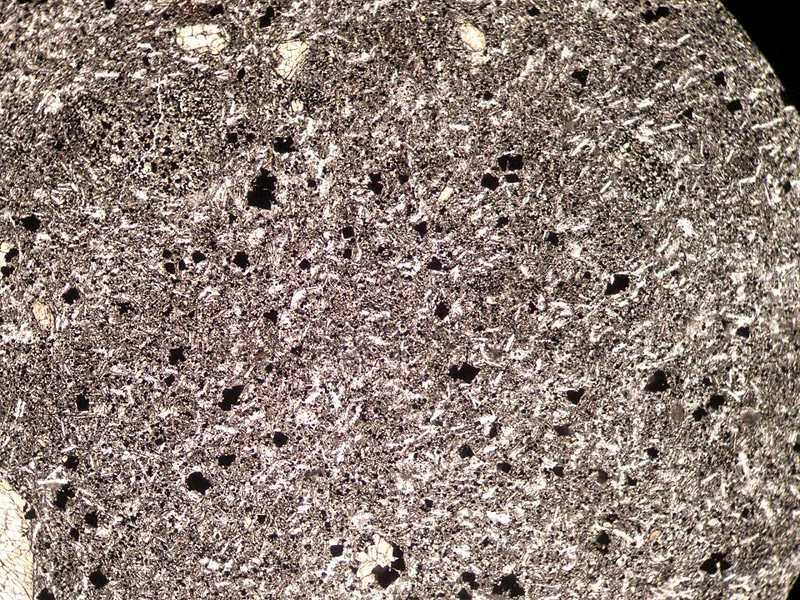
\includegraphics[height=3.6cm]{images/book2/g11-chmee2-basalt-ppl.jpg}\hfill
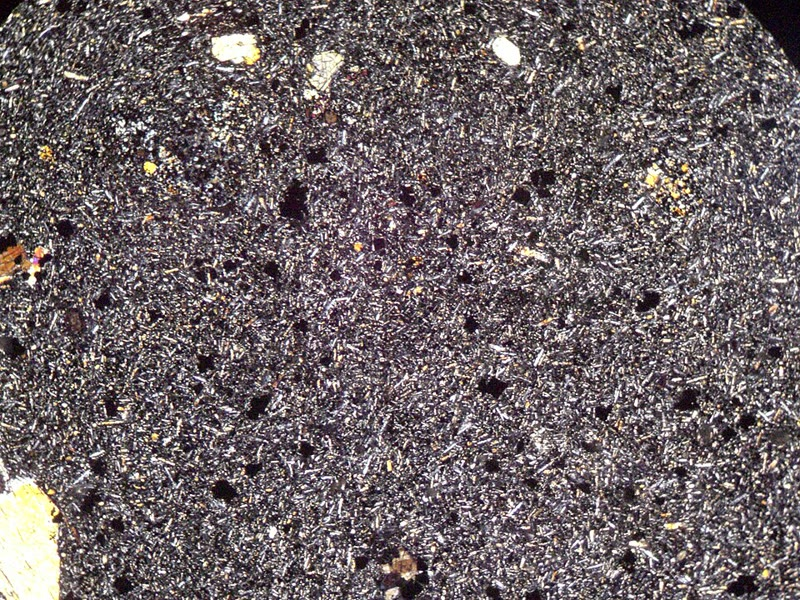
\includegraphics[height=3.6cm]{images/book2/g11-chmee2-basalt-xpl.jpg}\hfill
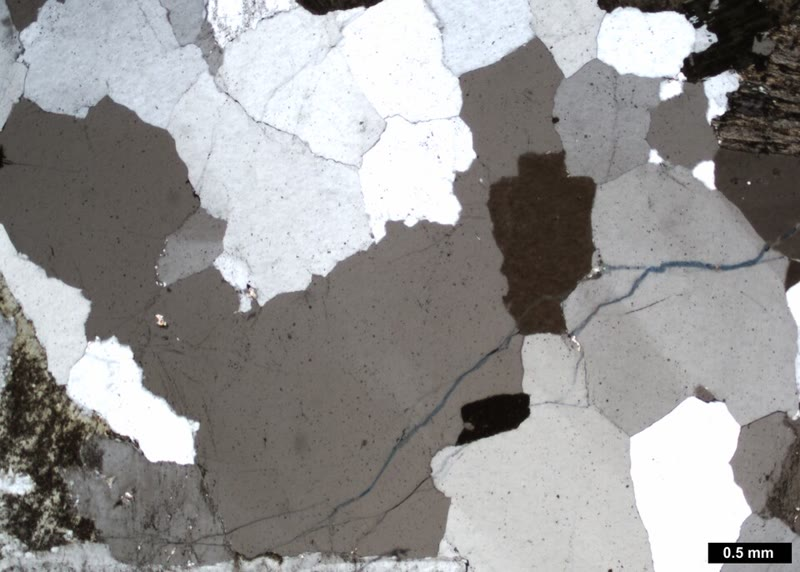
\includegraphics[height=3.6cm]{images/book2/g11-rygel-granite-xpl.jpg}

{\small बाएँ और बीच में: \omterm{def:g11:minerals:thin-section}{पतली काट} में वही बेसाल्ट, समतल-ध्रुवित
प्रकाश में और व्यत्यस्त ध्रुवकों के बीच। चट्टान बारीक कणों वाली है: छोटे लंबे
क्रिस्टल, ज़्यादातर प्लेजियोक्लेज़, और काले धब्बे जो किसी भी दृश्य में
कोई प्रकाश नहीं निकलने देते; व्यत्यस्त ध्रुवकों के बीच क्रिस्टल धूसर रंगतों और
रंगों में चमक उठते हैं। फ़ोटो
च्मी2 (CC~BY-SA~3.0)। दाएँ: एक ग्रेनाइट में क्वार्ट्ज़ के क्रिस्टल, व्यत्यस्त
ध्रुवकों के बीच, हर एक धूसर की अपनी रंगत में (पैमाना-पट्टी
\qty{0.5}{mm} है)। फ़ोटो माइकल सी॰~राइगल (CC~BY-SA~3.0)।}
\end{omfigure}
% ledger: photo:g11-basalt-thin-section, photo:g11-granite-thin-section

समतल-ध्रुवित प्रकाश में \omterm{def:g11:minerals:thin-section}{पतली काट} रंगीन काँच की खिड़की जैसी दिखती है:
अधिकांश खनिज लगभग रंगहीन होते हैं, कुछ हल्के रंगे हुए, और कणों की
रूपरेखाएँ, उनके \omterm{def:g11:minerals:cleavage}{विदलन} और उनके \omterm{def:g11:minerals:habit}{स्वभाव} साफ़ दिखते हैं। व्यत्यस्त
ध्रुवकों के बीच, एक-दूसरे के आड़े रखे फ़िल्टर अपने आप कोई प्रकाश
नहीं निकलने देते; अधिकांश खनिज अपने आर-पार जाने वाले प्रकाश को बदल देते हैं, और
धूसर रंगतों में या चटकीले रंगों में दिखते हैं, जो स्लाइड घुमाने पर बदलते हैं।
एक ही खनिज के दो कण अलग दिख सकते हैं, क्योंकि हर एक अपनी दिशा में
कटा है: ऊपर के ग्रेनाइट के क्वार्ट्ज़ कण सब क्वार्ट्ज़ हैं,
अलग-अलग रंगतों में। रंग, वे कैसे बदलते हैं, और वे हर खनिज के बारे में क्या प्रकट
करते हैं, ये विश्वविद्यालय के पहले वर्ष के विषय हैं; यहाँ
\omterm{def:g11:minerals:thin-section}{पतली काट} चट्टान का एक चित्र है, जिसमें हर कण देखा,
नामित और गिना जा सकता है।

\section{अभ्यास}

\begin{exercise}[$\star$]\label{exo:g11:minerals:1}
\omterm{def:g11:minerals:cleavage}{विदलन} और \omterm{def:g11:minerals:cleavage}{विभंग} की परिभाषा दीजिए। क्वार्ट्ज़ इनमें से कौन-सा दिखाता है, और उसकी
टूटी सतहें कैसी दिखती हैं? अभ्रक के कितने \omterm{def:g11:minerals:cleavage}{विदलन} होते हैं?
\end{exercise}

\begin{exercise}[$\star$]\label{exo:g11:minerals:2}
क्वार्ट्ज़ की पहचान के लिए रंग एक कमज़ोर मार्गदर्शक क्यों है, पर
ओलिवीन के लिए काफ़ी अच्छा? रंग से अधिक भरोसेमंद दो गुण बताइए।
\end{exercise}

\begin{exercise}[$\star$]\label{exo:g11:minerals:3}
हर वर्णन को क्वार्ट्ज़, ऑर्थोक्लेज़, बायोटाइट और
ओलिवीन में से किसी खनिज से मिलाइए: (1) बेसाल्ट में हरे कण; (2) काली पपड़ियाँ जो पतली
परतों में उतरती हैं; (3) दो समतल टूटन-तलों वाले गुलाबी खंड जैसे कण, जिन्हें
स्टील की कील खरोंच देती है; (4) वक्र टूटन वाले काँच जैसे धूसर कण, जिन्हें
कील नहीं खरोंचती।
\end{exercise}

\begin{exercise}[$\star$]\label{exo:g11:minerals:4}
(1) \omterm{def:g11:minerals:silicate}{सिलिकन--ऑक्सीजन चतुष्फलक} में कितने परमाणु होते हैं, और वे कहाँ
होते हैं? (2) आयनों \ce{Si^4+} और \ce{O^2-} के आवेशों का उपयोग करके समूह \ce{SiO4} का
आवेश ज्ञात कीजिए।
\end{exercise}

\begin{exercise}[$\star$]\label{exo:g11:minerals:5}
\omterm{def:g11:minerals:rock-forming}{शैलकारी सिलिकेटों} के छह समूहों के नाम बताइए और हर एक के लिए बताइए कि
उसके चतुष्फलक कैसे जुड़े हैं।
\end{exercise}

\begin{exercise}[$\star\star$]\label{exo:g11:minerals:6}
सिलिकन और ऑक्सीजन के परमाणु द्रव्यमान \qty{28.085}{g/mol} और
\qty{15.999}{g/mol} हैं। (1) क्वार्ट्ज़,
\ce{SiO2}, के द्रव्यमान में ऑक्सीजन का अंश परिकलित कीजिए। (2) यही फ़ॉर्स्टेराइट के लिए कीजिए, जो मैग्नीशियम ओलिवीन
\ce{Mg2SiO4} है (मैग्नीशियम: \qty{24.305}{g/mol})। (3) महाद्वीपीय भूपर्पटी में
ऑक्सीजन के अंश, लगभग \qty{46}{\percent}, से तुलना कीजिए।
\end{exercise}

\begin{exercise}[$\star\star$]\label{exo:g11:minerals:7}
ग्रेनाइट का एक सफ़ेद कण काँच की प्लेट (लगभग 5.5) को खरोंचता है पर
स्टील की कील (लगभग 6.5) से खरोंचा जाता है; वह दो दिशाओं में समतल तलों के अनुदिश
टूटता है। एक दूसरा, धूसर कण कील से नहीं खरोंचा जाता और
वक्र सतहों के अनुदिश टूटता है। दोनों को पहचानिए, कारण बताते हुए।
\end{exercise}

\begin{exercise}[$\star\star$]\label{exo:g11:minerals:8}
पाइरॉक्सीन ऑजाइट में हर चतुष्फलक दो कोने साझा करता है। (1)
ऑक्सीजनों की गिनती वाले प्रस्ताव का उपयोग करके बताइए कि हर सिलिकन के लिए कितने ऑक्सीजन
हैं? (2) जाँचिए कि ऑजाइट के सूत्र का भाग \ce{(Si,Al)2O6}
इससे मेल खाता है।
\end{exercise}

\begin{exercise}[$\star\star$]\label{exo:g11:minerals:9}
एक बेसाल्ट आयतन के अनुसार \qty{55}{\percent} लैब्राडोराइट (\qty{2.69}{g/cm^3}),
\qty{35}{\percent} ऑजाइट (\qty{3.4}{g/cm^3}) और \qty{10}{\percent} ओलिवीन
(\qty{3.32}{g/cm^3}) से बना है। उसका घनत्व परिकलित कीजिए, फिर
\qty{10}{cm} भुजा वाले इस बेसाल्ट के एक घन का द्रव्यमान।
\end{exercise}

\begin{exercise}[$\star\star$]\label{exo:g11:minerals:10}
प्रावार का एक \omterm{def:g11:ocean-ridges:peridotite}{पेरिडोटाइट} \qty{75}{\percent} ओलिवीन
(\qty{3.32}{g/cm^3}) और \qty{25}{\percent} ऑजाइट (\qty{3.4}{g/cm^3}) से बना है।
(1) उसका घनत्व परिकलित कीजिए। (2) वह पिछले अभ्यास के बेसाल्ट से,
जो लगभग \qty{3.00}{g/cm^3} का है, कितने प्रतिशत अधिक घना है? (3)
\omterm{def:g11:ocean-ridges:oceanic-lithosphere}{महासागरीय भूपर्पटी} प्रावार के ऊपर क्यों टिकी रहती है?
\end{exercise}

\begin{exercise}[$\star\star$]\label{exo:g11:minerals:11}
किसी चट्टान की \omterm{def:g11:minerals:thin-section}{पतली काट} पर 400 बिंदुओं का एक जाल 168 बार
प्लेजियोक्लेज़ पर, 132 बार पाइरॉक्सीन पर, 60 बार ओलिवीन पर और 40 बार
गैस के बुलबुलों द्वारा छोड़े गए छिद्रों पर पड़ता है। (1) हर एक का अंश परिकलित कीजिए। (2)
चट्टान के घनत्व वाला प्रस्ताव पूरी काट पर सीधे क्यों लागू नहीं किया जा
सकता? (3) \qty{2.69}{},
\qty{3.4}{} और \qty{3.32}{g/cm^3} के साथ ठोस भाग का घनत्व परिकलित कीजिए, फिर छिद्रों सहित चट्टान का।
\end{exercise}

\begin{exercise}[$\star\star\star$]\label{exo:g11:minerals:12}
\qty{1}{kg} महाद्वीपीय भूपर्पटी में लगभग \qty{464}{g} ऑक्सीजन,
\qty{283}{g} सिलिकन, \qty{84}{g} ऐलुमिनियम, \qty{52}{g} लोहा,
\qty{46}{g} कैल्सियम, \qty{28}{g} मैग्नीशियम, \qty{23}{g} सोडियम और
\qty{15}{g} पोटैशियम है। परमाणु द्रव्यमान \qty{16.0}{},
\qty{28.1}{}, \qty{27.0}{}, \qty{55.8}{}, \qty{40.1}{}, \qty{24.3}{}, \qty{23.0}{} और
\qty{39.1}{g/mol} हैं। (1) हर तत्त्व के मोलों की संख्या परिकलित कीजिए। (2)
भूपर्पटी के परमाणुओं का कितना अंश ऑक्सीजन परमाणु है? (3) भूपर्पटी को
कभी-कभी ऑक्सीजन आयनों के संकुलन के रूप में क्यों वर्णित किया जाता है, जिसमें दूसरे तत्त्व
उनके बीच की जगहों में हों?
\end{exercise}

\begin{exercise}[$\star\star\star$]\label{exo:g11:minerals:13}
ऐम्फ़िबोल की द्वि-शृंखला में आधे चतुष्फलक दो कोने साझा करते हैं और
आधे तीन। (1) हर सिलिकन के लिए कितने ऑक्सीजन हैं? (2) परिणाम
चार सिलिकनों के लिए लिखिए। (3) हॉर्नब्लेंड के सूत्र,
\ce{Ca2[Mg4(Al,Fe)]Si7AlO22(OH)2}, में आठ में से एक चतुष्फलक में ऐलुमिनियम
सिलिकन का स्थान लेता है। जाँचिए कि सूत्र इससे मेल खाता है।
\end{exercise}

\begin{exercise}[$\star\star\star$]\label{exo:g11:minerals:14}
कैलिफ़ोर्निया के सिएरा नेवादा पर \num{6454} ग्रेनाइटी चट्टान-नमूनों का
औसत घनत्व \qty{2.69}{g/cm^3} है; यह पश्चिम में \qty{2.7}{g/cm^3} से ऊपर है,
और वहाँ \qty{2.6}{g/cm^3} से नीचे जहाँ ग्रेनाइट सिलिका
और पोटैशियम से सबसे समृद्ध है। \qty{20}{\percent} क्वार्ट्ज़
(\qty{2.62}{g/cm^3}), \qty{10}{\percent} ऑर्थोक्लेज़ (\qty{2.56}{}),
\qty{50}{\percent} ऑलिगोक्लेज़ (\qty{2.65}{}), \qty{10}{\percent} बायोटाइट
(\qty{3.09}{}) और \qty{10}{\percent} हॉर्नब्लेंड (\qty{3.23}{}) वाली चट्टान का घनत्व परिकलित कीजिए। इसकी तुलना
इस अध्याय के उदाहरण के ग्रेनाइट से कीजिए, और सिएरा नेवादा के दोनों भागों के
बीच के अंतर को समझाइए।
\end{exercise}

\begin{exercise}[$\star\star\star$]\label{exo:g11:minerals:15}
ऊपरी महाद्वीपीय भूपर्पटी में द्रव्यमान के अनुसार लगभग \qty{66.6}{\percent} \ce{SiO2}
है, समग्र महाद्वीपीय भूपर्पटी में \qty{60.6}{\percent}। (1)
\ce{SiO2} में सिलिकन के अंश (\qty{46.7}{\percent}) का उपयोग करके हर एक में
\ce{SiO2} में बँधे सिलिकन का अंश परिकलित कीजिए। (2) आप किन खनिजों के
नीचे की अपेक्षा ऊपरी भूपर्पटी में अधिक सामान्य होने की अपेक्षा करेंगे? (3) गहरी भूपर्पटी की तुलना में
ऊपरी भूपर्पटी के घनत्व के लिए इसका क्या अर्थ है?
\end{exercise}

\section{समस्या: एक ग्रेनाइट का घनत्व}

\begin{problem}[{सप्ताहांत समस्या --- बिंदु-गणना से घनत्व तक}]
\label{pb:g11:minerals:1}
% values (mineral_density.py): GRANITE_COUNT 150/175/125/30/20; rho_granite 2.6427;
% granite_air_g 264.27, granite_water_g 164.27; densities wm:densities; usgs91:sierra
गुलाबी ग्रेनाइट का एक खंड काटकर चमकाया जाता है। उसके खनिज पहचाने जाते हैं,
एक जाल पर गिने जाते हैं, और चट्टान का घनत्व परिकलित किया जाता है, फिर
तौलकर जाँचा जाता है।

\medskip
\noindent\textbf{भाग I --- खनिजों की पहचान।}
\begin{enumerate}
  \item कण A धूसर और काँच जैसे हैं, उनमें कोई समतल टूटन-सतह नहीं, केवल
        वक्र सतहें, और स्टील की कील उन्हें नहीं खरोंचती। वे कौन-सा खनिज
        हैं?
  \item कण B गुलाबी और खंड जैसे हैं, दो दिशाओं में समतल चमकीले तलों के अनुदिश
        टूटते हैं, काँच को खरोंचते हैं पर कील से खरोंचे जाते हैं। वे कौन-सा
        खनिज हैं, और मोह्स पैमाने पर उनकी कठोरता क्या है?
  \item कण C की कठोरता और \omterm{def:g11:minerals:cleavage}{विदलन} कण B जैसे हैं पर वे
        सफ़ेद हैं; विश्लेषण उनमें सोडियम और कैल्सियम पाता है, और कोई
        पोटैशियम नहीं। वे किस प्रकार के फ़ेल्डस्पार हैं?
  \item कण D काली पपड़ियाँ हैं, कण E चाँदी जैसी पपड़ियाँ; दोनों पतली
        परतों में उतरते हैं। वे कौन-से खनिज हैं, और उनकी संरचना की कौन-सी
        विशेषता परतों को समझाती है?
  \item A से E तक के खनिजों में से कौन-से ढाँचा \omterm{def:g11:minerals:silicate}{सिलिकेट} हैं? किनमें
        लोहा और मैग्नीशियम है?
\end{enumerate}

\medskip
\noindent\textbf{भाग II --- बिंदु-गणना।}
\begin{enumerate}[resume]
  \item 500 बिंदुओं का एक जाल 150 बार क्वार्ट्ज़ पर, 175 बार
        ऑर्थोक्लेज़ पर, 125 बार ऑलिगोक्लेज़ पर, 30 बार बायोटाइट पर और 20 बार
        मस्कोवाइट पर पड़ता है। हर खनिज का अंश परिकलित कीजिए।
  \item बिंदुओं का अंश चट्टान के आयतन के अंश का अनुमान क्यों
        देता है?
  \item चट्टान का कितना प्रतिशत फ़ेल्डस्पार है?
  \item यदि एक बिंदु गलत गिना जाए, तो कोई अंश कितना बदलता है?
  \item क्या यह चट्टान पुस्तक 1 के अर्थ में ग्रेनाइट है?
\end{enumerate}

\medskip
\noindent\textbf{भाग III --- घनत्व।}
\begin{enumerate}[resume]
  \item बिना रंध्रों की चट्टान का घनत्व उसके खनिजों से देने वाला सूत्र
        लिखिए।
  \item घनत्वों क्वार्ट्ज़ \qty{2.62}{}, ऑर्थोक्लेज़ \qty{2.56}{},
        ऑलिगोक्लेज़ \qty{2.65}{}, बायोटाइट \qty{3.09}{} और मस्कोवाइट
        \qty{2.82}{g/cm^3} के साथ हर खनिज का योगदान $\phi_i \rho_i$
        परिकलित कीजिए।
  \item इन्हें जोड़िए: ग्रेनाइट का घनत्व क्या है?
  \item कौन-सा खनिज योग में सबसे अधिक योगदान देता है? कौन-से दो खनिज,
        यद्यपि वे चट्टान का केवल दसवाँ भाग बनाते हैं, उसका घनत्व बढ़ाते हैं?
  \item घनत्व को \unit{kg/m^3} में बदलिए, और इस ग्रेनाइट के
        \qty{1}{m^3} का द्रव्यमान बताइए।
\end{enumerate}

\medskip
\noindent\textbf{भाग IV --- तौलकर जाँच।}
\begin{enumerate}[resume]
  \item ग्रेनाइट से \qty{100}{cm^3} का एक खंड काटा जाता है। आप उसके किस द्रव्यमान की
        अपेक्षा करते हैं?
  \item पानी में लटकाने पर किसी पिंड को उसके द्वारा हटाए गए पानी का भार ऊपर
        धकेलता है (भौतिकी)। जब खंड \qty{1.00}{g/cm^3} घनत्व वाले पानी में
        पूरा डूबा लटका हो, तो तुला कितना द्रव्यमान पढ़ती है?
  \item प्रयोगशालाएँ चट्टान के नमूने का घनत्व
        $m_{\text{वायु}}/(m_{\text{वायु}} - m_{\text{जल}})$ के रूप में परिकलित करती हैं। जाँचिए कि
        आपके दोनों द्रव्यमान प्रश्न~13 का घनत्व वापस देते हैं।
  \item सिएरा नेवादा की ग्रेनाइटी चट्टानों का औसत \qty{2.69}{g/cm^3} है, और
        सिलिका और पोटैशियम से सबसे समृद्ध चट्टानें \qty{2.6}{g/cm^3} से नीचे हैं।
        यह ग्रेनाइट कहाँ आता है, और कौन-से खनिज किसी
        ग्रेनाइट को अधिक घना बनाएँगे?
  \item निष्कर्ष निकालिए: ग्रेनाइट का घनत्व क्या है?
\end{enumerate}
\end{problem}
